\documentclass[12pt,a4paper]{report}

% IEEE-style packages
\usepackage[utf8]{inputenc}
\usepackage[T1]{fontenc}
\usepackage{times}
\usepackage{graphicx}
\usepackage{amsmath}
\usepackage{amssymb}
\usepackage{booktabs}
\usepackage{multirow}
\usepackage{array}
\usepackage{tabularx}
\usepackage{longtable}
\usepackage{float}
\usepackage{placeins}
\usepackage{caption}
\usepackage{subcaption}
\usepackage{hyperref}
\usepackage{xcolor}
\usepackage{listings}
\usepackage{tikz}
\usetikzlibrary{positioning, arrows.meta, shapes.geometric}

% Page layout
\usepackage[margin=1in]{geometry}
\usepackage{setspace}
\onehalfspacing

% Code listing style
\definecolor{codegreen}{rgb}{0,0.6,0}
\definecolor{codegray}{rgb}{0.5,0.5,0.5}
\definecolor{codepurple}{rgb}{0.58,0,0.82}
\definecolor{backcolour}{rgb}{0.95,0.95,0.92}

\lstdefinestyle{mystyle}{
    backgroundcolor=\color{backcolour},
    commentstyle=\color{codegreen},
    keywordstyle=\color{blue},
    numberstyle=\tiny\color{codegray},
    stringstyle=\color{codepurple},
    basicstyle=\ttfamily\footnotesize,
    breakatwhitespace=false,
    breaklines=true,
    captionpos=b,
    keepspaces=true,
    numbers=left,
    numbersep=5pt,
    showspaces=false,
    showstringspaces=false,
    showtabs=false,
    tabsize=2,
    frame=single,
    framesep=5pt,
    xleftmargin=15pt,
    xrightmargin=5pt
}
\lstset{style=mystyle}

% Define JavaScript language for listings
\lstdefinelanguage{JavaScript}{
    keywords={typeof, new, true, false, catch, function, return, null, catch, switch, var, let, const, if, in, while, do, else, case, break, async, await, try, throw, export, import, class, extends, interface, type},
    keywordstyle=\color{blue}\bfseries,
    ndkeywords={boolean, number, string, void, any, Promise, Array, Object},
    ndkeywordstyle=\color{codepurple}\bfseries,
    identifierstyle=\color{black},
    sensitive=true,
    comment=[l]{//},
    morecomment=[s]{/*}{*/},
    commentstyle=\color{codegreen}\ttfamily,
    stringstyle=\color{red}\ttfamily,
    morestring=[b]',
    morestring=[b]",
    morestring=[b]`
}

% Checkmark symbol
\usepackage{pifont}
\newcommand{\cmark}{\ding{51}}
\newcommand{\xmark}{\ding{55}}
\renewcommand{\checkmark}{\cmark}

% Header/Footer
\usepackage{fancyhdr}
\pagestyle{fancy}
\fancyhf{}
\fancyhead[L]{\leftmark}
\fancyhead[R]{\thepage}
\renewcommand{\headrulewidth}{0.4pt}

% Title information
\title{
    \textbf{Pixelar: An AI-Powered Game Asset Generation Platform}\\
    \vspace{0.5cm}
    \large Chapters 1-3: Introduction, Literature Review, and Architecture
}
\author{
    Final Year Project Report\\
    \vspace{0.3cm}
    Department of Computer Science
}
\date{\today}

\begin{document}

% Title page
\maketitle

% Table of contents
\tableofcontents
\listoffigures
\listoftables
\lstlistoflistings

\newpage

% Include chapters 1, 2, and 3 only
\chapter{Introduction}
\label{chap:introduction}

\section{Overview}

The video game industry has experienced unprecedented growth over the past decade, with the global market valued at \$217.06 billion in 2024 and projected to reach \$363.2 billion by 2032. This expansion has been accompanied by an increasing demand for high-quality visual assets, including character sprites, environmental backgrounds, and animations. Traditionally, the creation of these assets has been a labor-intensive process requiring specialized artistic skills, expensive software tools, and significant time investment.

The emergence of generative artificial intelligence (AI) technologies, particularly diffusion models and large language models (LLMs), has opened new possibilities for automating creative processes. Models such as Stable Diffusion, DALL-E, and Midjourney have demonstrated remarkable capabilities in generating photorealistic and stylized images from textual descriptions. However, these general-purpose tools often fall short when applied to the specific requirements of game development, where assets must adhere to particular artistic styles, maintain consistency across multiple generations, and meet technical specifications for integration into game engines.

Pixelar addresses this gap by providing a specialized AI-powered platform designed explicitly for game asset generation. The system leverages state-of-the-art generative models while incorporating domain-specific optimizations for pixel art, 2D flat styles, and animation sequences. By combining advanced prompt engineering techniques with a user-friendly interface, Pixelar democratizes game asset creation, enabling developers of all skill levels to produce professional-quality visual content efficiently.

The platform operates on a Software-as-a-Service (SaaS) model, offering both credit-based usage of platform-hosted AI models and a Bring Your Own Key (BYOK) option for users who prefer to use their personal API credentials. This flexible approach accommodates diverse user needs, from hobbyist game developers working on small projects to professional studios requiring high-volume asset generation.

\section{Project Motivation}

The motivation for developing Pixelar stems from several critical observations and challenges in the current game development landscape:

\subsection{The Asset Creation Bottleneck}

Game development projects frequently encounter delays due to the time-consuming nature of asset creation. A single character sprite with multiple animation frames can require 8-16 hours of work from a skilled pixel artist. For indie developers and small studios operating with limited budgets and tight deadlines, this represents a significant bottleneck that can delay project completion or force compromises in visual quality.

According to a 2023 survey by the International Game Developers Association (IGDA), 67\% of indie developers identified ``art and asset creation'' as their primary development challenge, surpassing even programming and game design concerns. This finding underscores the pressing need for tools that can accelerate the asset creation pipeline without sacrificing quality.

\subsection{The Skills Gap}

Many game developers possess strong programming abilities but lack formal training in visual arts. This skills gap forces developers to either:
\begin{itemize}
    \item Invest significant time in learning artistic techniques
    \item Hire freelance artists or outsource asset creation
    \item Use generic asset packs that may not align with their creative vision
    \item Compromise on visual quality by using placeholder or low-quality assets
\end{itemize}

Each of these alternatives presents drawbacks in terms of time, cost, or creative control. An AI-powered generation tool can bridge this gap by translating textual descriptions into visual assets, allowing developers to realize their creative vision without requiring advanced artistic skills.

\subsection{Limitations of Existing Tools}

While several AI image generation tools exist, they exhibit significant limitations when applied to game asset creation:

\begin{enumerate}
    \item \textbf{Lack of Style Consistency}: General-purpose generators struggle to maintain consistent artistic styles across multiple generations, making it difficult to create cohesive asset sets.
    
    \item \textbf{No Animation Support}: Most existing tools generate static images only, requiring separate workflows for creating animation sequences.
    
    \item \textbf{Inappropriate Output Formats}: Generated images often include backgrounds, artifacts, or dimensions unsuitable for direct use in game engines.
    
    \item \textbf{Limited Viewpoint Control}: Game assets frequently require specific viewpoints (isometric, top-down, side-scrolling) that general tools do not adequately support.
    
    \item \textbf{No Project Organization}: Existing tools lack features for organizing generated assets into projects, tracking generation history, or managing asset metadata.
\end{enumerate}

\subsection{Economic Considerations}

The cost of professional game art can be prohibitive for independent developers. Commissioned character sprites typically range from \$50-200 per character, with animated sprites commanding even higher prices. A complete set of assets for a modest 2D game can easily exceed \$5,000-10,000, representing a significant barrier to entry for hobbyist and indie developers.

AI-powered generation offers a cost-effective alternative, with per-asset costs measured in cents rather than dollars. This economic advantage can democratize game development by making professional-quality assets accessible to developers regardless of their budget constraints.

\clearpage
\section{Project Vision, Scope, and Glossary}

\subsection{Vision Statement}

Pixelar envisions a future where creative vision is the only limitation in game development. By harnessing the power of artificial intelligence, the platform aims to eliminate technical and financial barriers to asset creation, enabling developers worldwide to bring their game concepts to life with professional-quality visual content.

The platform aspires to become the industry-standard tool for AI-assisted game asset generation, continuously evolving to incorporate advances in generative AI while maintaining its focus on the specific needs of game developers.

\subsection{Project Scope}

The scope of Pixelar encompasses the following functional areas:

\subsubsection{In-Scope Features}

\begin{enumerate}
    \item \textbf{Sprite Generation}
    \begin{itemize}
        \item Character sprites with customizable attributes
        \item Object and item sprites
        \item Multiple art styles (pixel art, 2D flat)
        \item Various viewpoints (front, side, isometric, top-down)
        \item Configurable dimensions and aspect ratios
        \item Color palette specification
    \end{itemize}
    
    \item \textbf{Scene Generation}
    \begin{itemize}
        \item Indoor and outdoor environments
        \item Background scenes for various game genres
        \item Tileable patterns for seamless backgrounds
        \item Multiple aspect ratios for different platforms
    \end{itemize}
    
    \item \textbf{Animation Generation}
    \begin{itemize}
        \item Character animation sequences
        \item 47 predefined animation actions
        \item Frame-by-frame generation with character consistency
        \item Sprite sheet assembly and export
        \item GIF conversion functionality
    \end{itemize}
    
    \item \textbf{Project Management}
    \begin{itemize}
        \item Project creation and organization
        \item Asset categorization and tagging
        \item Generation history tracking
        \item Metadata storage for reproducibility
    \end{itemize}
    
    \item \textbf{User Management}
    \begin{itemize}
        \item User authentication and authorization
        \item Credit-based billing system
        \item BYOK (Bring Your Own Key) support
        \item User profile management
    \end{itemize}
\end{enumerate}

\subsubsection{Out-of-Scope Features}

The following features are explicitly excluded from the current project scope:

\begin{itemize}
    \item 3D model generation
    \item Audio and sound effect generation
    \item Game engine integration plugins
    \item Collaborative multi-user editing
    \item Mobile application development
    \item Offline generation capabilities
\end{itemize}

\subsection{Glossary of Terms}

\noindent
\begin{minipage}{\textwidth}
\centering
\captionof{table}{Glossary of Technical Terms}
\label{tab:glossary}
\small
\begin{tabular}{|l|p{9cm}|}
\hline
\textbf{Term} & \textbf{Definition} \\
\hline
API & Application Programming Interface; a set of protocols enabling software components to communicate \\
\hline
BYOK & Bring Your Own Key; a feature allowing users to use their personal API credentials \\
\hline
CDN & Content Delivery Network; distributed servers for fast content delivery \\
\hline
Diffusion Model & A type of generative AI model that creates images by iteratively denoising random noise \\
\hline
Firebase & Google's platform for mobile and web application development \\
\hline
Firestore & Firebase's NoSQL document database \\
\hline
GIF & Graphics Interchange Format; an image format supporting animation \\
\hline
Isometric & A method of visual representation using a 45-degree angle projection \\
\hline
JWT & JSON Web Token; a compact token format for secure information transmission \\
\hline
LLM & Large Language Model; AI models trained on vast text corpora \\
\hline
Pixel Art & A digital art form where images are created at the pixel level \\
\hline
Prompt Engineering & The practice of crafting effective inputs for AI models \\
\hline
REST API & Representational State Transfer API; an architectural style for web services \\
\hline
SaaS & Software as a Service; cloud-based software delivery model \\
\hline
Sprite & A 2D image or animation integrated into a larger scene \\
\hline
Sprite Sheet & A single image containing multiple sprites arranged in a grid \\
\hline
\end{tabular}
\end{minipage}
\vspace{0.5cm}

\clearpage
\section{Objectives}

The development of Pixelar is guided by the following primary and secondary objectives:

\subsection{Primary Objectives}

\begin{enumerate}
    \item \textbf{Develop a Functional AI-Powered Generation Platform}
    \begin{itemize}
        \item Implement sprite generation with $>$95\% success rate
        \item Achieve average generation time under 15 seconds
        \item Support multiple art styles and viewpoints
        \item Enable color palette customization
    \end{itemize}
    
    \item \textbf{Implement Animation Generation Capabilities}
    \begin{itemize}
        \item Create frame-by-frame animation generation pipeline
        \item Achieve $>$85\% character consistency across frames
        \item Support at least 40 predefined animation actions
        \item Enable sprite sheet export functionality
    \end{itemize}
    
    \item \textbf{Build a Robust Backend Infrastructure}
    \begin{itemize}
        \item Design scalable API architecture
        \item Implement secure user authentication
        \item Create efficient database schema for asset management
        \item Integrate cloud storage for generated assets
    \end{itemize}
    
    \item \textbf{Develop an Intuitive User Interface}
    \begin{itemize}
        \item Create responsive web application
        \item Implement real-time generation feedback
        \item Design accessible and user-friendly controls
        \item Support project organization features
    \end{itemize}
\end{enumerate}

\subsection{Secondary Objectives}

\begin{enumerate}
    \item \textbf{Implement Multi-Provider AI Support}
    \begin{itemize}
        \item Integrate Replicate API for primary generation
        \item Add Google Gemini API as fallback provider
        \item Enable seamless provider switching
    \end{itemize}
    
    \item \textbf{Create Flexible Billing System}
    \begin{itemize}
        \item Implement credit-based usage tracking
        \item Support BYOK for cost-conscious users
        \item Provide transparent usage reporting
    \end{itemize}
    
    \item \textbf{Ensure System Reliability}
    \begin{itemize}
        \item Achieve $>$99.5\% system uptime
        \item Implement error handling and recovery
        \item Create comprehensive logging and monitoring
    \end{itemize}
    
    \item \textbf{Optimize Generation Quality}
    \begin{itemize}
        \item Develop effective prompt engineering templates
        \item Achieve user satisfaction score $>$4.0/5.0
        \item Minimize generation artifacts and errors
    \end{itemize}
\end{enumerate}

\subsection{Success Criteria}

The project will be considered successful upon meeting the following measurable criteria:

\noindent
\begin{minipage}{\textwidth}
\centering
\captionof{table}{Project Success Criteria}
\label{tab:success_criteria}
\begin{tabular}{|l|c|l|}
\hline
\textbf{Criterion} & \textbf{Target} & \textbf{Measurement Method} \\
\hline
Generation Success Rate & $>$95\% & Automated logging \\
\hline
Average Response Time & $<$15 seconds & Performance monitoring \\
\hline
System Uptime & $>$99.5\% & Uptime tracking service \\
\hline
User Satisfaction & $>$4.0/5.0 & User surveys \\
\hline
Animation Consistency & $>$85\% & SSIM analysis \\
\hline
Test Coverage & $>$90\% & Code coverage tools \\
\hline
\end{tabular}
\end{minipage}
\vspace{0.5cm}

\clearpage
\section{Tools and Technologies}

The development of Pixelar utilizes a carefully selected technology stack optimized for performance, scalability, and developer productivity.

\subsection{Frontend Technologies}

\noindent
\begin{minipage}{\textwidth}
\centering
\captionof{table}{Frontend Technology Stack}
\label{tab:frontend_tech}
\begin{tabular}{|l|l|p{6.5cm}|}
\hline
\textbf{Technology} & \textbf{Version} & \textbf{Purpose} \\
\hline
Next.js & 15.5.6 & React framework with server-side rendering, routing, and optimization \\
\hline
React & 18.x & Component-based UI library for building interactive interfaces \\
\hline
TypeScript & 5.x & Typed superset of JavaScript for improved code quality \\
\hline
Tailwind CSS & 3.4.x & Utility-first CSS framework for rapid UI development \\
\hline
Lucide React & Latest & Icon library providing consistent visual elements \\
\hline
\end{tabular}
\end{minipage}
\vspace{0.5cm}

\subsection{Backend Technologies}

\noindent
\begin{minipage}{\textwidth}
\centering
\captionof{table}{Backend Technology Stack}
\label{tab:backend_tech}
\begin{tabular}{|l|l|p{6.5cm}|}
\hline
\textbf{Technology} & \textbf{Version} & \textbf{Purpose} \\
\hline
Node.js & 20.x LTS & JavaScript runtime for server-side execution \\
\hline
Express.js & 4.x & Minimal web framework for API development \\
\hline
TypeScript & 5.x & Type-safe backend development \\
\hline
Firebase Admin SDK & 12.x & Server-side Firebase services access \\
\hline
\end{tabular}
\end{minipage}
\vspace{0.5cm}

\subsection{Database and Storage}

\noindent
\begin{minipage}{\textwidth}
\centering
\captionof{table}{Database and Storage Technologies}
\label{tab:database_tech}
\begin{tabular}{|l|l|p{6.5cm}|}
\hline
\textbf{Technology} & \textbf{Version} & \textbf{Purpose} \\
\hline
Firebase Firestore & Latest & NoSQL document database for user data, projects, and assets \\
\hline
Vercel Blob & 0.23.x & Cloud object storage for generated images with CDN \\
\hline
Firebase Auth & 10.x & User authentication and session management \\
\hline
\end{tabular}
\end{minipage}
\vspace{0.5cm}

\subsection{AI and Generation Services}

\noindent
\begin{minipage}{\textwidth}
\centering
\captionof{table}{AI Service Providers}
\label{tab:ai_tech}
\begin{tabular}{|l|p{9cm}|}
\hline
\textbf{Service} & \textbf{Purpose} \\
\hline
Replicate API & Primary AI generation provider; hosts custom-trained models optimized for game assets \\
\hline
Google Gemini API & Secondary provider; offers fast generation with multimodal capabilities \\
\hline
\end{tabular}
\end{minipage}
\vspace{0.5cm}

\subsection{Development Tools}

\noindent
\begin{minipage}{\textwidth}
\centering
\captionof{table}{Development and Deployment Tools}
\label{tab:dev_tools}
\begin{tabular}{|l|p{9cm}|}
\hline
\textbf{Tool} & \textbf{Purpose} \\
\hline
Visual Studio Code & Primary integrated development environment \\
\hline
Git & Version control system \\
\hline
GitHub & Code repository and collaboration platform \\
\hline
Vercel & Frontend deployment and hosting platform \\
\hline
Railway & Backend deployment platform \\
\hline
Postman & API testing and documentation \\
\hline
Jest & JavaScript testing framework \\
\hline
ESLint & Code linting and style enforcement \\
\hline
Prettier & Code formatting \\
\hline
\end{tabular}
\end{minipage}
\vspace{0.5cm}

\subsection{Technology Selection Rationale}

The technology stack was selected based on the following criteria:

\begin{enumerate}
    \item \textbf{Performance}: Next.js provides server-side rendering and automatic code splitting, ensuring fast page loads. Node.js offers non-blocking I/O ideal for handling concurrent API requests.
    
    \item \textbf{Scalability}: Firebase Firestore automatically scales to handle increased load. Vercel's edge network ensures global content delivery with minimal latency.
    
    \item \textbf{Developer Experience}: TypeScript catches errors at compile time, reducing runtime bugs. Tailwind CSS accelerates UI development with utility classes.
    
    \item \textbf{Cost Efficiency}: Firebase and Vercel offer generous free tiers suitable for development and initial deployment. Pay-as-you-go pricing scales with usage.
    
    \item \textbf{Ecosystem}: The selected technologies have large communities, extensive documentation, and abundant third-party libraries.
    
    \item \textbf{Integration}: All components integrate seamlessly, with official SDKs and well-documented APIs facilitating development.
\end{enumerate}
\chapter{Background Study and Literature Review}
\label{chap:literature}

This chapter presents a comprehensive review of the existing literature and related work in the domains of AI-powered image generation, game asset creation tools, and animation synthesis. The review establishes the theoretical foundation for the Pixelar platform and identifies gaps in current solutions that the project aims to address.

\section{Theoretical Background}

\subsection{Generative Artificial Intelligence}

Generative AI refers to artificial intelligence systems capable of creating new content, including text, images, audio, and video. Unlike discriminative models that classify or predict based on input data, generative models learn the underlying distribution of training data and can produce novel samples from that distribution.

The field has evolved through several paradigm shifts:

\subsubsection{Generative Adversarial Networks (GANs)}

Introduced by Goodfellow et al. in 2014, GANs consist of two neural networks—a generator and a discriminator—trained in an adversarial manner. The generator creates synthetic samples while the discriminator attempts to distinguish real from generated samples. This adversarial training process drives both networks to improve, ultimately producing highly realistic outputs.

GANs have been successfully applied to image generation tasks, with variants such as StyleGAN achieving remarkable results in generating photorealistic human faces. However, GANs suffer from training instability, mode collapse, and difficulty in controlling specific attributes of generated outputs.

\subsubsection{Variational Autoencoders (VAEs)}

VAEs provide a probabilistic approach to generative modeling by learning a latent representation of input data. The encoder maps inputs to a latent space, while the decoder reconstructs outputs from latent representations. VAEs offer more stable training than GANs but typically produce blurrier outputs.

\subsubsection{Diffusion Models}

Diffusion models represent the current state-of-the-art in image generation. These models learn to reverse a gradual noising process, starting from pure noise and iteratively denoising to produce coherent images. Key advantages include:

\begin{itemize}
    \item Stable training without adversarial dynamics
    \item High-quality, diverse outputs
    \item Controllable generation through conditioning
    \item Scalability to high resolutions
\end{itemize}

Notable diffusion-based systems include Stable Diffusion, DALL-E 2, and Midjourney. These models have demonstrated unprecedented capabilities in generating images from textual descriptions, enabling creative applications previously impossible.

\subsubsection{Transformer-Based Models}

The transformer architecture, originally developed for natural language processing, has been adapted for image generation through models like Vision Transformer (ViT). Google's Gemini represents a multimodal transformer capable of processing and generating both text and images, offering unique capabilities for understanding complex prompts and generating contextually appropriate outputs.

\subsection{Prompt Engineering}

Prompt engineering has emerged as a critical discipline in leveraging generative AI effectively. The quality and specificity of input prompts significantly influence generation outcomes. Key principles include:

\begin{enumerate}
    \item \textbf{Specificity}: Detailed descriptions yield more accurate results than vague prompts.
    \item \textbf{Structure}: Organized prompts with clear sections (subject, style, composition) improve consistency.
    \item \textbf{Negative Prompts}: Specifying what to avoid helps eliminate unwanted elements.
    \item \textbf{Style References}: Including artistic style keywords guides aesthetic choices.
    \item \textbf{Technical Parameters}: Specifying dimensions, aspect ratios, and quality levels ensures appropriate outputs.
\end{enumerate}

Research has demonstrated that well-engineered prompts can improve generation quality by 30-50\% compared to naive prompts, highlighting the importance of this technique in practical applications.

\subsection{Game Asset Creation}

Game assets encompass all visual, audio, and data elements used in video game development. Visual assets specifically include:

\begin{itemize}
    \item \textbf{Sprites}: 2D images representing characters, objects, and environmental elements
    \item \textbf{Tilesets}: Collections of tiles for constructing game levels
    \item \textbf{Backgrounds}: Static or parallax scrolling environmental imagery
    \item \textbf{UI Elements}: Buttons, icons, and interface components
    \item \textbf{Animations}: Sequences of frames depicting motion
\end{itemize}

Traditional asset creation workflows involve specialized software such as Adobe Photoshop, Aseprite, or Pyxel Edit, requiring significant artistic skill and time investment. A professional pixel artist typically produces 2-4 finished sprites per day, with complex animated characters requiring multiple days of work.

\subsection{Animation Principles}

Animation in games follows principles established by Disney animators, adapted for the constraints of real-time rendering:

\begin{enumerate}
    \item \textbf{Squash and Stretch}: Exaggerating deformation to convey weight and flexibility
    \item \textbf{Anticipation}: Preparatory movements before main actions
    \item \textbf{Staging}: Clear presentation of actions for readability
    \item \textbf{Follow Through}: Continuation of movement after main action
    \item \textbf{Timing}: Spacing of frames to convey speed and weight
\end{enumerate}

Game animations must balance these principles against technical constraints including frame count limitations, memory usage, and real-time performance requirements.

\clearpage
\section{Related Work}

\subsection{General-Purpose AI Image Generators}

\subsubsection{DALL-E and DALL-E 2}

OpenAI's DALL-E systems pioneered text-to-image generation using transformer and diffusion architectures. DALL-E 2 generates 1024×1024 images with impressive photorealism and creative interpretation of prompts.

\textbf{Strengths}: High-quality photorealistic outputs, strong prompt understanding, inpainting and outpainting capabilities.

\textbf{Limitations for Game Development}: No specific support for pixel art or game styles, limited control over exact dimensions, no animation capabilities, closed API with usage restrictions.

\subsubsection{Midjourney}

Midjourney has gained popularity for its artistic quality and distinctive aesthetic. Operating through Discord, it offers an accessible interface for creative image generation.

\textbf{Strengths}: Exceptional artistic quality, strong community and style sharing, intuitive variation and upscaling features.

\textbf{Limitations for Game Development}: Discord-only interface unsuitable for integration, no API access for automated workflows, limited style consistency across generations, no game-specific optimizations.

\subsubsection{Stable Diffusion}

Stable Diffusion represents an open-source diffusion model enabling local deployment and customization. Its accessibility has spawned numerous derivative tools and fine-tuned models.

\textbf{Strengths}: Open-source and customizable, extensive community models and extensions, local deployment option, ControlNet for pose guidance.

\textbf{Limitations for Game Development}: Requires technical expertise for optimal results, inconsistent quality without fine-tuning, resource-intensive local deployment, no integrated project management.

\subsection{Game-Specific Asset Generation Tools}

\subsubsection{Scenario.gg}

Scenario provides AI-powered asset generation specifically for game developers. It offers custom model training and game-focused generation features.

\textbf{Strengths}: Game-focused feature set, custom model training, style consistency tools, API access for integration.

\textbf{Limitations}: Limited animation support, higher pricing tier for advanced features, requires model training for optimal results, no BYOK option.

\subsubsection{Leonardo.AI}

Leonardo.AI offers AI image generation with features tailored for creative professionals, including game developers.

\textbf{Strengths}: Multiple fine-tuned models, canvas editing features, texture generation capabilities.

\textbf{Limitations}: Limited pixel art optimization, no dedicated animation pipeline, complex interface for beginners, subscription-based pricing only.

\subsubsection{PixelLab}

PixelLab focuses specifically on pixel art generation, offering style-consistent outputs for retro game aesthetics.

\textbf{Strengths}: Pixel art specialization, consistent retro aesthetics, simple interface.

\textbf{Limitations}: Limited to pixel art style only, no animation support, basic feature set, no project organization.

\subsection{Animation Generation Systems}

\subsubsection{GodModeAI}

GodModeAI represents a specialized system for generating character animations from static images. It offers predefined animation actions and frame-by-frame generation.

\textbf{Strengths}: Comprehensive animation action library, character consistency focus, isometric view support, auto-repose functionality.

\textbf{Limitations}: Animation-only focus (no sprite/scene generation), limited style customization, no project management features, single provider dependency.

\subsubsection{Animated Drawings by Meta}

Meta's Animated Drawings project enables animation of children's drawings through pose estimation and rigging.

\textbf{Strengths}: Novel approach to animation, works with hand-drawn inputs, open-source implementation.

\textbf{Limitations}: Limited to simple character animations, requires specific input format, not optimized for game assets, no generation capabilities.

\subsection{Traditional Asset Creation Tools}

\subsubsection{Aseprite}

Aseprite is the industry-standard tool for pixel art creation and animation. It provides comprehensive features for manual asset creation.

\textbf{Strengths}: Professional-grade pixel art tools, comprehensive animation timeline, layer and frame management, export to multiple formats.

\textbf{Limitations}: Requires artistic skill, time-intensive workflow, no AI assistance, steep learning curve.

\subsubsection{Pyxel Edit}

Pyxel Edit offers tileset-focused pixel art creation with animation support.

\textbf{Strengths}: Tileset optimization, animation preview, affordable pricing.

\textbf{Limitations}: Manual creation only, limited advanced features, no AI integration.

\clearpage
\section{Comparative Analysis}

\noindent
\begin{minipage}{\textwidth}
\centering
\captionof{table}{Comprehensive Feature Comparison of Related Tools}
\label{tab:feature_comparison}
\small
\begin{tabular}{|l|c|c|c|c|c|c|}
\hline
\textbf{Feature} & \textbf{DALL-E} & \textbf{Midjourney} & \textbf{Scenario} & \textbf{Leonardo} & \textbf{GodMode} & \textbf{Pixelar} \\
\hline
Sprite Generation & Partial & Partial & \checkmark & \checkmark & $\times$ & \checkmark \\
\hline
Scene Generation & \checkmark & \checkmark & \checkmark & \checkmark & $\times$ & \checkmark \\
\hline
Animation & $\times$ & $\times$ & $\times$ & $\times$ & \checkmark & \checkmark \\
\hline
Pixel Art Style & $\times$ & Partial & \checkmark & Partial & \checkmark & \checkmark \\
\hline
Isometric View & $\times$ & $\times$ & Partial & $\times$ & \checkmark & \checkmark \\
\hline
BYOK Support & $\times$ & $\times$ & $\times$ & $\times$ & $\times$ & \checkmark \\
\hline
Multi-Provider & $\times$ & $\times$ & $\times$ & $\times$ & $\times$ & \checkmark \\
\hline
Project Mgmt & $\times$ & $\times$ & \checkmark & Partial & $\times$ & \checkmark \\
\hline
API Access & \checkmark & $\times$ & \checkmark & \checkmark & Partial & \checkmark \\
\hline
Free Tier & Limited & $\times$ & Limited & \checkmark & Limited & \checkmark \\
\hline
\end{tabular}
\end{minipage}
\vspace{0.5cm}

\section{Research Gaps and Limitations}

The literature review reveals several significant gaps in existing solutions:

\subsection{Integration Gap}

No existing tool provides a unified platform combining sprite generation, scene creation, and animation synthesis. Users must employ multiple tools and manage complex workflows to produce complete asset sets. This fragmentation increases development time and introduces consistency challenges.

\subsection{Flexibility Gap}

Current solutions lock users into specific AI providers and pricing models. The absence of BYOK options forces users to accept platform pricing regardless of their usage patterns or existing API subscriptions. This inflexibility particularly disadvantages high-volume users and those with existing provider relationships.

\subsection{Animation Consistency Gap}

While tools like GodModeAI address animation generation, maintaining character consistency across frames remains challenging. Existing approaches often produce noticeable variations in character appearance, requiring manual correction or multiple generation attempts.

\subsection{Game-Specific Optimization Gap}

General-purpose generators lack optimizations for game asset requirements:
\begin{itemize}
    \item Transparent backgrounds for sprite integration
    \item Specific viewpoints (isometric, top-down) common in games
    \item Appropriate dimensions for various game engines
    \item Style consistency across asset collections
\end{itemize}

\subsection{Project Management Gap}

Most generation tools focus solely on image creation without supporting the broader asset management workflow. Features such as project organization, generation history, metadata tracking, and asset categorization are typically absent or rudimentary.

\subsection{Accessibility Gap}

Many advanced tools require significant technical expertise or artistic knowledge to use effectively. This creates barriers for indie developers and hobbyists who could benefit most from AI-assisted asset creation.

\clearpage
\section{Addressing the Gaps: Pixelar's Approach}

Pixelar addresses the identified gaps through the following design decisions:

\begin{enumerate}
    \item \textbf{Unified Platform}: Integrating sprite, scene, and animation generation in a single application eliminates workflow fragmentation and ensures consistent user experience.
    
    \item \textbf{Multi-Provider Architecture}: Supporting both Replicate and Gemini APIs with BYOK capability provides flexibility in provider selection and cost management.
    
    \item \textbf{Character Reference Injection}: Passing character images as references during animation frame generation improves consistency by providing explicit visual guidance to the AI model.
    
    \item \textbf{Game-Optimized Prompts}: Developing specialized prompt templates incorporating game-specific requirements (viewpoints, styles, dimensions) ensures outputs suitable for direct use in game engines.
    
    \item \textbf{Comprehensive Project Management}: Including project organization, asset categorization, and metadata storage supports complete asset management workflows.
    
    \item \textbf{Intuitive Interface}: Designing an accessible interface with guided workflows enables users of all skill levels to generate professional-quality assets.
\end{enumerate}

\section{Theoretical Framework}

The development of Pixelar is grounded in the following theoretical frameworks:

\subsection{Human-AI Collaboration Model}

Pixelar adopts a collaborative model where AI augments rather than replaces human creativity. Users provide creative direction through prompts and parameters while AI handles technical execution. This approach preserves creative control while eliminating technical barriers.

\subsection{Iterative Refinement Process}

The platform supports iterative refinement through:
\begin{itemize}
    \item Multiple generation attempts with varied parameters
    \item Reference image guidance for style consistency
    \item Prompt modification based on initial results
    \item Selective regeneration of unsatisfactory outputs
\end{itemize}

This aligns with established creative workflows where initial concepts are progressively refined toward final outputs.

\subsection{Modular Architecture Pattern}

The system architecture follows modular design principles, separating concerns into distinct components:
\begin{itemize}
    \item Generation service (AI provider abstraction)
    \item Storage service (blob management)
    \item User service (authentication and profiles)
    \item Project service (asset organization)
\end{itemize}

This modularity enables independent evolution of components and facilitates testing and maintenance.

\section{Summary}

This literature review has examined the current state of AI-powered image generation, game asset creation tools, and animation synthesis systems. While significant advances have been made in generative AI capabilities, existing tools exhibit limitations in integration, flexibility, consistency, and game-specific optimization.

Pixelar addresses these gaps by providing a unified platform combining sprite, scene, and animation generation with multi-provider support, BYOK capability, and comprehensive project management. The platform's design is grounded in established theoretical frameworks for human-AI collaboration, iterative refinement, and modular architecture.

The following chapters detail the system requirements, architecture, and implementation of Pixelar, demonstrating how these design decisions translate into a functional platform that advances the state of AI-assisted game asset creation.
\chapter{System Requirements, Architecture and Design}
\label{chap:architecture}

This chapter presents the comprehensive system requirements, architectural design, and development plan for the Pixelar platform.

\clearpage
\section{System Requirements}

\subsection{Functional Requirements}

The functional requirements define the specific behaviors and functions that the Pixelar system must provide.

\subsubsection{User Management Requirements}

\noindent
\begin{minipage}{\textwidth}
\centering
\captionof{table}{User Management Functional Requirements}
\label{tab:fr_user}
\small
\begin{tabular}{|l|p{7cm}|c|}
\hline
\textbf{ID} & \textbf{Requirement} & \textbf{Priority} \\
\hline
FR-U01 & Allow users to register using email and password & High \\
\hline
FR-U02 & Support Google OAuth authentication & High \\
\hline
FR-U03 & Maintain user sessions using JWT tokens & High \\
\hline
FR-U04 & Allow users to view and edit their profile & Medium \\
\hline
FR-U05 & Track user credit balance & High \\
\hline
FR-U06 & Support BYOK API key storage (client-side) & Medium \\
\hline
\end{tabular}
\end{minipage}
\vspace{0.5cm}

\subsubsection{Generation Requirements}

\noindent
\begin{minipage}{\textwidth}
\centering
\captionof{table}{Asset Generation Functional Requirements}
\label{tab:fr_gen}
\small
\begin{tabular}{|l|p{7cm}|c|}
\hline
\textbf{ID} & \textbf{Requirement} & \textbf{Priority} \\
\hline
FR-G01 & Generate sprite images from text prompts & High \\
\hline
FR-G02 & Support pixel art and 2D flat styles & High \\
\hline
FR-G03 & Support multiple viewpoints & High \\
\hline
FR-G04 & Allow color palette specification & Medium \\
\hline
FR-G05 & Generate scene/background images & High \\
\hline
FR-G06 & Generate animation frame sequences & High \\
\hline
FR-G07 & Maintain character consistency across frames & High \\
\hline
FR-G08 & Support 47 predefined animation actions & Medium \\
\hline
FR-G09 & Allow reference image upload & Medium \\
\hline
FR-G10 & Support multiple aspect ratios & Medium \\
\hline
\end{tabular}
\end{minipage}
\vspace{0.5cm}

\subsubsection{Project Management Requirements}

\noindent
\begin{minipage}{\textwidth}
\centering
\captionof{table}{Project Management Functional Requirements}
\label{tab:fr_project}
\small
\begin{tabular}{|l|p{7cm}|c|}
\hline
\textbf{ID} & \textbf{Requirement} & \textbf{Priority} \\
\hline
FR-P01 & Allow users to create projects & High \\
\hline
FR-P02 & Allow users to organize assets within projects & High \\
\hline
FR-P03 & Track generation history with metadata & Medium \\
\hline
FR-P04 & Allow project deletion (soft delete) & Medium \\
\hline
FR-P05 & Display recent sessions on dashboard & Low \\
\hline
\end{tabular}
\end{minipage}
\vspace{0.5cm}

\subsubsection{Export Requirements}

\noindent
\begin{minipage}{\textwidth}
\centering
\captionof{table}{Export Functional Requirements}
\label{tab:fr_export}
\small
\begin{tabular}{|l|p{7cm}|c|}
\hline
\textbf{ID} & \textbf{Requirement} & \textbf{Priority} \\
\hline
FR-E01 & Allow downloading individual generated images & High \\
\hline
FR-E02 & Generate sprite sheets from animation frames & High \\
\hline
FR-E03 & Convert sprite sheets to animated GIFs & Medium \\
\hline
FR-E04 & Support PNG format with transparency & High \\
\hline
\end{tabular}
\end{minipage}
\vspace{0.5cm}

\clearpage
\subsection{Non-Functional Requirements}

\subsubsection{Performance Requirements}

\noindent
\begin{minipage}{\textwidth}
\centering
\captionof{table}{Performance Non-Functional Requirements}
\label{tab:nfr_perf}
\small
\begin{tabular}{|l|p{6cm}|c|}
\hline
\textbf{ID} & \textbf{Requirement} & \textbf{Target} \\
\hline
NFR-P01 & Average sprite generation time & $<$ 15 seconds \\
\hline
NFR-P02 & API response time (non-generation) & $<$ 500 ms \\
\hline
NFR-P03 & Page load time & $<$ 3 seconds \\
\hline
NFR-P04 & Concurrent user support & $>$ 100 users \\
\hline
NFR-P05 & Image upload time & $<$ 2 seconds \\
\hline
\end{tabular}
\end{minipage}
\vspace{0.5cm}

\subsubsection{Reliability Requirements}

\noindent
\begin{minipage}{\textwidth}
\centering
\captionof{table}{Reliability Non-Functional Requirements}
\label{tab:nfr_rel}
\small
\begin{tabular}{|l|p{6cm}|c|}
\hline
\textbf{ID} & \textbf{Requirement} & \textbf{Target} \\
\hline
NFR-R01 & System uptime & $>$ 99.5\% \\
\hline
NFR-R02 & Generation success rate & $>$ 95\% \\
\hline
NFR-R03 & Data backup frequency & Daily \\
\hline
NFR-R04 & Mean time to recovery & $<$ 1 hour \\
\hline
\end{tabular}
\end{minipage}
\vspace{0.5cm}

\subsubsection{Security Requirements}

\noindent
\begin{minipage}{\textwidth}
\centering
\captionof{table}{Security Non-Functional Requirements}
\label{tab:nfr_sec}
\small
\begin{tabular}{|l|p{9cm}|}
\hline
\textbf{ID} & \textbf{Requirement} \\
\hline
NFR-S01 & All API endpoints require authentication except public routes \\
\hline
NFR-S02 & User passwords hashed using industry-standard algorithms \\
\hline
NFR-S03 & BYOK API keys stored client-side only, never on server \\
\hline
NFR-S04 & All data transmission uses HTTPS encryption \\
\hline
NFR-S05 & JWT tokens expire after 1 hour \\
\hline
\end{tabular}
\end{minipage}
\vspace{0.5cm}

\subsubsection{Usability Requirements}

\noindent
\begin{minipage}{\textwidth}
\centering
\captionof{table}{Usability Non-Functional Requirements}
\label{tab:nfr_use}
\small
\begin{tabular}{|l|p{9cm}|}
\hline
\textbf{ID} & \textbf{Requirement} \\
\hline
NFR-U01 & Interface responsive across desktop and tablet devices \\
\hline
NFR-U02 & Users generate first asset within 5 minutes of registration \\
\hline
NFR-U03 & Error messages are clear and actionable \\
\hline
NFR-U04 & Visual feedback provided during generation processes \\
\hline
\end{tabular}
\end{minipage}
\vspace{0.5cm}

\clearpage
\section{System Flow Chart}

The following flow chart illustrates the primary user workflow for generating game assets.

\noindent
\begin{minipage}{\textwidth}
\centering
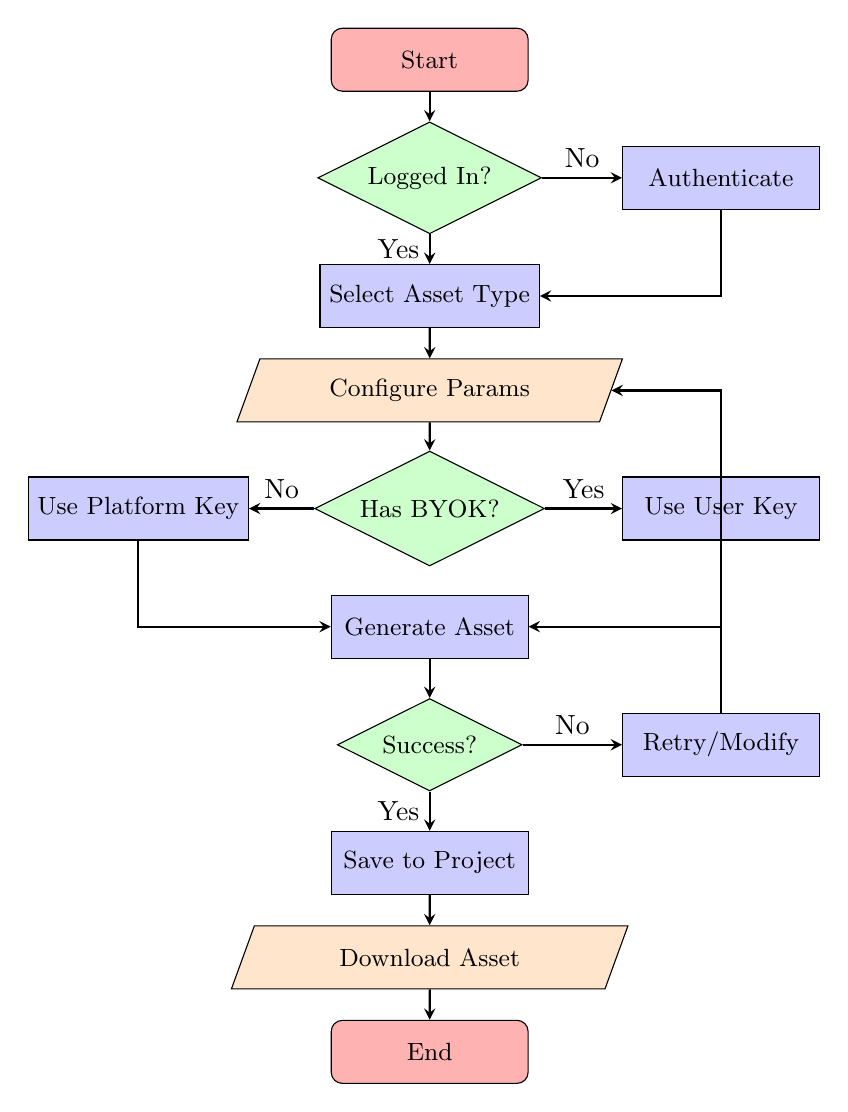
\begin{tikzpicture}[
    node distance=1.2cm,
    startstop/.style={rectangle, rounded corners, minimum width=2.5cm, minimum height=0.8cm, text centered, draw=black, fill=red!30, font=\small},
    process/.style={rectangle, minimum width=2.5cm, minimum height=0.8cm, text centered, draw=black, fill=blue!20, font=\small},
    decision/.style={diamond, minimum width=2cm, minimum height=0.8cm, text centered, draw=black, fill=green!20, aspect=2, font=\small},
    io/.style={trapezium, trapezium left angle=70, trapezium right angle=110, minimum width=2.5cm, minimum height=0.8cm, text centered, draw=black, fill=orange!20, font=\small},
    arrow/.style={thick,->,>=stealth}
]

\node (start) [startstop] {Start};
\node (login) [decision, below of=start, yshift=-0.3cm] {Logged In?};
\node (auth) [process, right of=login, xshift=2.5cm] {Authenticate};
\node (select) [process, below of=login, yshift=-0.3cm] {Select Asset Type};
\node (config) [io, below of=select] {Configure Params};
\node (haskey) [decision, below of=config, yshift=-0.3cm] {Has BYOK?};
\node (usebyok) [process, right of=haskey, xshift=2.5cm] {Use User Key};
\node (useplatform) [process, left of=haskey, xshift=-2.5cm] {Use Platform Key};
\node (generate) [process, below of=haskey, yshift=-0.3cm] {Generate Asset};
\node (success) [decision, below of=generate, yshift=-0.3cm] {Success?};
\node (retry) [process, right of=success, xshift=2.5cm] {Retry/Modify};
\node (save) [process, below of=success, yshift=-0.3cm] {Save to Project};
\node (download) [io, below of=save] {Download Asset};
\node (end) [startstop, below of=download] {End};

\draw [arrow] (start) -- (login);
\draw [arrow] (login) -- node[anchor=south] {No} (auth);
\draw [arrow] (auth) |- (select);
\draw [arrow] (login) -- node[anchor=east] {Yes} (select);
\draw [arrow] (select) -- (config);
\draw [arrow] (config) -- (haskey);
\draw [arrow] (haskey) -- node[anchor=south] {Yes} (usebyok);
\draw [arrow] (haskey) -- node[anchor=south] {No} (useplatform);
\draw [arrow] (usebyok) |- (generate);
\draw [arrow] (useplatform) |- (generate);
\draw [arrow] (generate) -- (success);
\draw [arrow] (success) -- node[anchor=south] {No} (retry);
\draw [arrow] (retry) |- (config);
\draw [arrow] (success) -- node[anchor=east] {Yes} (save);
\draw [arrow] (save) -- (download);
\draw [arrow] (download) -- (end);

\end{tikzpicture}
\captionof{figure}{Asset Generation Flow Chart}
\label{fig:flowchart}
\end{minipage}
\vspace{0.5cm}

\subsection{Detailed Process Flows}

\textbf{Sprite Generation Flow:}
\begin{enumerate}
    \item User navigates to Sprite Generator page
    \item User selects sprite type (Character/Object)
    \item User enters text prompt describing desired sprite
    \item User configures parameters (style, viewpoint, aspect ratio, colors)
    \item System validates user credits or BYOK key
    \item System constructs optimized prompt and calls AI API
    \item System uploads images to blob storage and saves metadata
    \item User previews, downloads, or saves to project
\end{enumerate}

\textbf{Animation Generation Flow:}
\begin{enumerate}
    \item User uploads character image
    \item User selects animation action from library (47 actions)
    \item User configures view type and direction
    \item System generates each frame with character reference
    \item System assembles frames into animation preview
    \item User exports as sprite sheet or GIF
\end{enumerate}

\clearpage
\section{Use Case Diagram}

\noindent
\begin{minipage}{\textwidth}
\centering
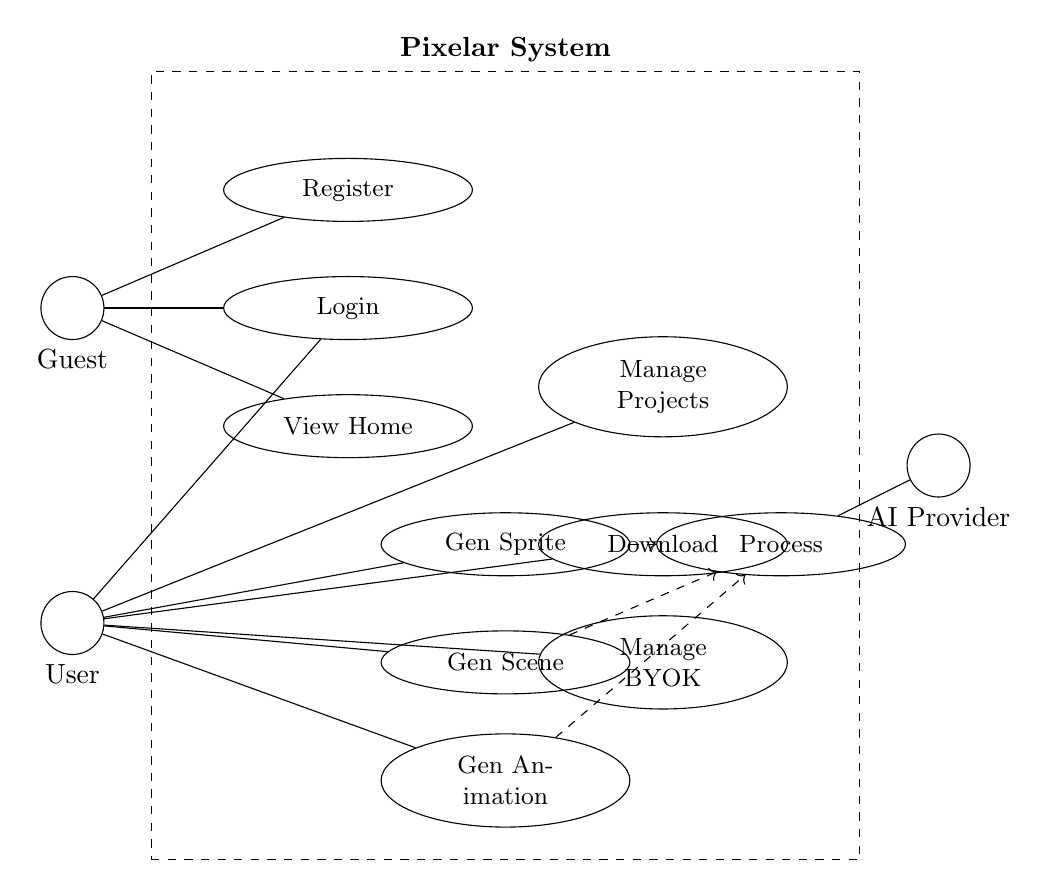
\begin{tikzpicture}[
    actor/.style={circle, draw, minimum size=0.8cm, font=\small},
    usecase/.style={ellipse, draw, minimum width=2cm, minimum height=0.8cm, text centered, text width=2cm, font=\small},
    system/.style={rectangle, draw, dashed, minimum width=9cm, minimum height=10cm}
]

\node[system, label=above:{\textbf{Pixelar System}}] (system) at (4.5,0) {};

\node[actor, label=below:{Guest}] (guest) at (-1, 2) {};
\node[actor, label=below:{User}] (user) at (-1, -2) {};
\node[actor, label=below:{AI Provider}] (ai) at (10, 0) {};

\node[usecase] (register) at (2.5, 3.5) {Register};
\node[usecase] (login) at (2.5, 2) {Login};
\node[usecase] (viewhome) at (2.5, 0.5) {View Home};
\node[usecase] (gensprite) at (4.5, -1) {Gen Sprite};
\node[usecase] (genscene) at (4.5, -2.5) {Gen Scene};
\node[usecase] (genanim) at (4.5, -4) {Gen Animation};
\node[usecase] (manageproj) at (6.5, 1) {Manage Projects};
\node[usecase] (download) at (6.5, -1) {Download};
\node[usecase] (managebyok) at (6.5, -2.5) {Manage BYOK};
\node[usecase] (processgen) at (8, -1) {Process};

\draw (guest) -- (register);
\draw (guest) -- (login);
\draw (guest) -- (viewhome);
\draw (user) -- (login);
\draw (user) -- (gensprite);
\draw (user) -- (genscene);
\draw (user) -- (genanim);
\draw (user) -- (manageproj);
\draw (user) -- (download);
\draw (user) -- (managebyok);
\draw (ai) -- (processgen);

\draw[dashed, ->] (gensprite) -- (processgen);
\draw[dashed, ->] (genscene) -- (processgen);
\draw[dashed, ->] (genanim) -- (processgen);

\end{tikzpicture}
\captionof{figure}{Use Case Diagram}
\label{fig:usecase}
\end{minipage}
\vspace{0.5cm}

\clearpage
\subsection{Use Case Descriptions}

\noindent
\begin{minipage}{\textwidth}
\centering
\captionof{table}{Use Case: Generate Sprite (UC-01)}
\label{tab:uc_sprite}
\small
\begin{tabular}{|p{3cm}|p{9cm}|}
\hline
\textbf{Use Case ID} & UC-01 \\
\hline
\textbf{Name} & Generate Sprite \\
\hline
\textbf{Actor} & Authenticated User \\
\hline
\textbf{Description} & User generates sprite images using AI based on text prompts \\
\hline
\textbf{Preconditions} & User logged in; has credits or BYOK key \\
\hline
\textbf{Postconditions} & Sprites saved; credits deducted (if applicable) \\
\hline
\textbf{Main Flow} & 
1. Navigate to Sprite Generator \newline
2. Enter prompt and configure parameters \newline
3. Click Generate \newline
4. System validates and calls AI \newline
5. System displays generated sprites \newline
6. User downloads or saves to project \\
\hline
\textbf{Alternative Flow} & 
A1. Insufficient credits: Show error \newline
A2. Generation fails: Allow retry \\
\hline
\end{tabular}
\end{minipage}
\vspace{0.5cm}

\noindent
\begin{minipage}{\textwidth}
\centering
\captionof{table}{Use Case: Generate Animation (UC-02)}
\label{tab:uc_anim}
\small
\begin{tabular}{|p{3cm}|p{9cm}|}
\hline
\textbf{Use Case ID} & UC-02 \\
\hline
\textbf{Name} & Generate Animation \\
\hline
\textbf{Actor} & Authenticated User \\
\hline
\textbf{Description} & User generates animation frame sequences from character image \\
\hline
\textbf{Preconditions} & User logged in; has character image; has credits/BYOK \\
\hline
\textbf{Postconditions} & Animation frames saved; sprite sheet available \\
\hline
\textbf{Main Flow} & 
1. Upload character image \newline
2. Select animation action \newline
3. Configure view and direction \newline
4. System generates frames sequentially \newline
5. System displays animation preview \newline
6. User exports sprite sheet or GIF \\
\hline
\end{tabular}
\end{minipage}
\vspace{0.5cm}

\noindent
\begin{minipage}{\textwidth}
\centering
\captionof{table}{Use Case: Manage Projects (UC-03)}
\label{tab:uc_project}
\small
\begin{tabular}{|p{3cm}|p{9cm}|}
\hline
\textbf{Use Case ID} & UC-03 \\
\hline
\textbf{Name} & Manage Projects \\
\hline
\textbf{Actor} & Authenticated User \\
\hline
\textbf{Description} & User creates, views, updates, and deletes projects \\
\hline
\textbf{Preconditions} & User is logged in \\
\hline
\textbf{Postconditions} & Project changes persisted to database \\
\hline
\textbf{Main Flow} & 
1. Navigate to Projects page \newline
2. View list of existing projects \newline
3. Create new or select existing project \newline
4. View project details and assets \newline
5. Update or delete project \\
\hline
\end{tabular}
\end{minipage}
\vspace{0.5cm}

\clearpage
\section{Software Development Plan}

\subsection{The Software Architecture}

The Pixelar platform follows a modern three-tier architecture with clear separation of concerns.

\subsubsection{High-Level Architecture}

\noindent
\begin{minipage}{\textwidth}
\centering
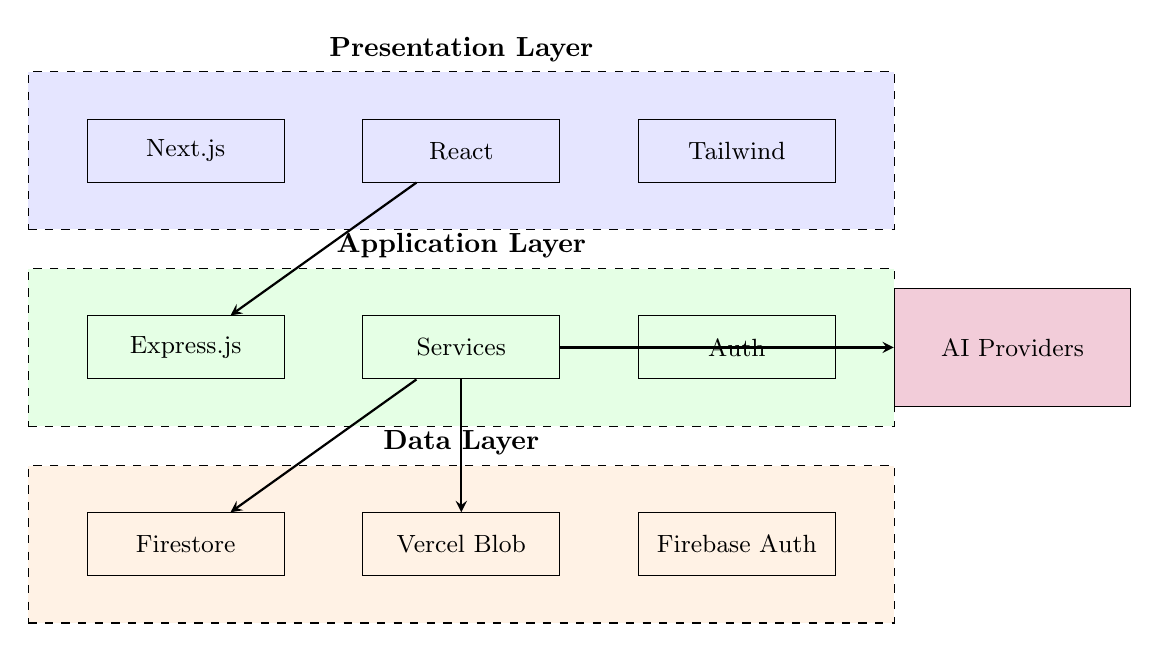
\begin{tikzpicture}[
    box/.style={rectangle, draw, minimum width=2.5cm, minimum height=0.8cm, text centered, font=\small},
    bigbox/.style={rectangle, draw, minimum width=3cm, minimum height=1.5cm, text centered, font=\small},
    layer/.style={rectangle, draw, dashed, minimum width=11cm, minimum height=2cm},
    arrow/.style={thick, ->, >=stealth}
]

\node[layer, fill=blue!10, label=above:{\textbf{Presentation Layer}}] (pres) at (0, 5) {};
\node[layer, fill=green!10, label=above:{\textbf{Application Layer}}] (app) at (0, 2.5) {};
\node[layer, fill=orange!10, label=above:{\textbf{Data Layer}}] (data) at (0, 0) {};

\node[box] (nextjs) at (-3.5, 5) {Next.js};
\node[box] (react) at (0, 5) {React};
\node[box] (tailwind) at (3.5, 5) {Tailwind};

\node[box] (express) at (-3.5, 2.5) {Express.js};
\node[box] (services) at (0, 2.5) {Services};
\node[box] (auth) at (3.5, 2.5) {Auth};

\node[box] (firestore) at (-3.5, 0) {Firestore};
\node[box] (blob) at (0, 0) {Vercel Blob};
\node[box] (firebase) at (3.5, 0) {Firebase Auth};

\node[bigbox, fill=purple!20] (ai) at (7, 2.5) {AI Providers};

\draw[arrow] (react) -- (express);
\draw[arrow] (services) -- (firestore);
\draw[arrow] (services) -- (blob);
\draw[arrow] (services) -- (ai);

\end{tikzpicture}
\captionof{figure}{High-Level System Architecture}
\label{fig:architecture}
\end{minipage}
\vspace{0.5cm}

\subsubsection{Frontend Architecture}

The frontend follows a component-based architecture using React and Next.js:

\begin{lstlisting}[language=bash, caption={Frontend Directory Structure}]
frontend/
├── app/           # Next.js App Router pages
├── components/    # Reusable UI components
├── contexts/      # React context providers
├── hooks/         # Custom React hooks
├── lib/           # Utility functions
└── public/        # Static assets
\end{lstlisting}

\subsubsection{Backend Architecture}

The backend implements a service-oriented architecture:

\begin{lstlisting}[language=bash, caption={Backend Directory Structure}]
Backend/
├── api/
│   ├── index.ts       # Express entry point
│   └── routes/        # API route handlers
├── services/          # Business logic
├── lib/               # Shared utilities
├── types/             # TypeScript definitions
└── tests/             # Test suite
\end{lstlisting}

\clearpage
\subsubsection{Database Schema Design}

\noindent
\begin{minipage}{\textwidth}
\centering
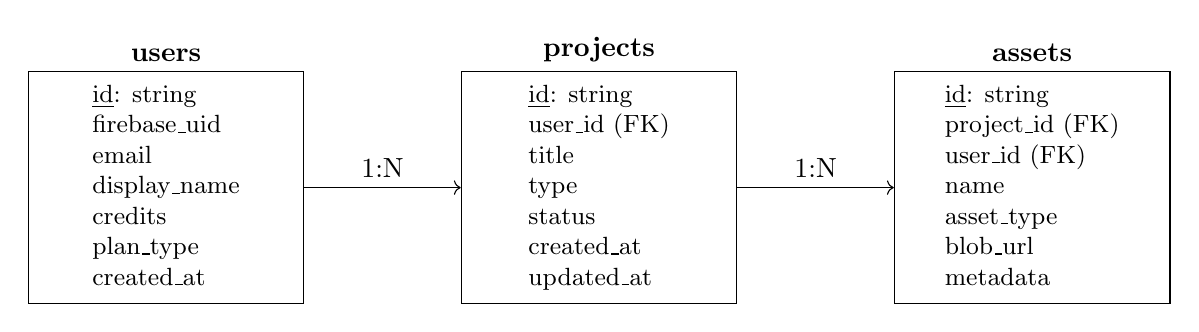
\begin{tikzpicture}[
    entity/.style={rectangle, draw, minimum width=3.5cm, minimum height=2.5cm, text centered, font=\small}
]

\node[entity, label=above:{\textbf{users}}] (users) at (0, 0) {
    \begin{tabular}{l}
    \underline{id}: string \\
    firebase\_uid \\
    email \\
    display\_name \\
    credits \\
    plan\_type \\
    created\_at
    \end{tabular}
};

\node[entity, label=above:{\textbf{projects}}] (projects) at (5.5, 0) {
    \begin{tabular}{l}
    \underline{id}: string \\
    user\_id (FK) \\
    title \\
    type \\
    status \\
    created\_at \\
    updated\_at
    \end{tabular}
};

\node[entity, label=above:{\textbf{assets}}] (assets) at (11, 0) {
    \begin{tabular}{l}
    \underline{id}: string \\
    project\_id (FK) \\
    user\_id (FK) \\
    name \\
    asset\_type \\
    blob\_url \\
    metadata
    \end{tabular}
};

\draw[->] (users.east) -- node[above] {1:N} (projects.west);
\draw[->] (projects.east) -- node[above] {1:N} (assets.west);

\end{tikzpicture}
\captionof{figure}{Database Entity Relationship Diagram}
\label{fig:erd}
\end{minipage}
\vspace{0.5cm}

\subsubsection{API Architecture}

\noindent
\begin{minipage}{\textwidth}
\centering
\captionof{table}{API Endpoint Architecture}
\label{tab:api_arch}
\small
\begin{tabular}{|l|l|l|p{4.5cm}|}
\hline
\textbf{Method} & \textbf{Endpoint} & \textbf{Auth} & \textbf{Description} \\
\hline
\multicolumn{4}{|c|}{\textbf{Generation Endpoints}} \\
\hline
POST & /api/generate/sprite & Yes & Generate sprite images \\
\hline
POST & /api/generate/scene & Yes & Generate scene images \\
\hline
POST & /api/generate/animation & Yes & Generate animation frames \\
\hline
GET & /api/generate/history & Yes & Get generation history \\
\hline
\multicolumn{4}{|c|}{\textbf{User Endpoints}} \\
\hline
GET & /api/user/profile & Yes & Get user profile \\
\hline
PUT & /api/user/profile & Yes & Update user profile \\
\hline
POST & /api/user/credits/deduct & Yes & Deduct credits \\
\hline
\multicolumn{4}{|c|}{\textbf{Project Endpoints}} \\
\hline
GET & /api/projects & Yes & List user projects \\
\hline
POST & /api/projects & Yes & Create project \\
\hline
GET & /api/projects/:id & Yes & Get project details \\
\hline
PUT & /api/projects/:id & Yes & Update project \\
\hline
DELETE & /api/projects/:id & Yes & Delete project \\
\hline
\end{tabular}
\end{minipage}
\vspace{0.5cm}

\clearpage
\subsection{Number of Development Iterations}

The project was developed using Agile Scrum methodology in four two-week iterations.

\noindent
\begin{minipage}{\textwidth}
\centering
\captionof{table}{Development Iteration Summary}
\label{tab:iterations}
\small
\begin{tabular}{|c|l|c|c|l|}
\hline
\textbf{Iter.} & \textbf{Focus Area} & \textbf{Duration} & \textbf{Semester} & \textbf{Status} \\
\hline
1 & Core Infrastructure & 2 weeks & 7 & Completed \\
\hline
2 & AI Generation Service & 2 weeks & 7 & Completed \\
\hline
3 & Animation System & 2 weeks & 8 & Completed \\
\hline
4 & Project Management & 2 weeks & 8 & Completed \\
\hline
\end{tabular}
\end{minipage}
\vspace{0.5cm}

\subsubsection{Iteration 1: Core Infrastructure (Semester 7)}

\textbf{Duration}: Weeks 1-2

\textbf{Objectives}: Establish project structure, implement authentication, design database schema, create frontend shell.

\noindent
\begin{minipage}{\textwidth}
\centering
\captionof{table}{Iteration 1 Sprint Backlog}
\label{tab:sprint1}
\small
\begin{tabular}{|p{6cm}|c|c|}
\hline
\textbf{Task} & \textbf{Points} & \textbf{Status} \\
\hline
Set up Next.js project structure & 3 & Done \\
\hline
Set up Express.js backend & 3 & Done \\
\hline
Implement Firebase Auth integration & 5 & Done \\
\hline
Create authentication middleware & 3 & Done \\
\hline
Design Firestore schema & 5 & Done \\
\hline
Implement User Service & 5 & Done \\
\hline
Create login/register pages & 5 & Done \\
\hline
Implement profile management & 3 & Done \\
\hline
Set up Vercel deployment & 2 & Done \\
\hline
Write unit tests & 5 & Done \\
\hline
\textbf{Total} & \textbf{39} & \\
\hline
\end{tabular}
\end{minipage}
\vspace{0.5cm}

\subsubsection{Iteration 2: AI Generation Service (Semester 7)}

\textbf{Duration}: Weeks 3-4

\textbf{Objectives}: Integrate AI providers, implement prompt engineering, create generation endpoints, implement BYOK.

\noindent
\begin{minipage}{\textwidth}
\centering
\captionof{table}{Iteration 2 Sprint Backlog}
\label{tab:sprint2}
\small
\begin{tabular}{|p{6cm}|c|c|}
\hline
\textbf{Task} & \textbf{Points} & \textbf{Status} \\
\hline
Integrate Replicate API & 8 & Done \\
\hline
Integrate Gemini API (fallback) & 5 & Done \\
\hline
Implement provider abstraction & 5 & Done \\
\hline
Develop prompt engineering system & 8 & Done \\
\hline
Create sprite generation endpoint & 5 & Done \\
\hline
Create scene generation endpoint & 5 & Done \\
\hline
Implement BYOK frontend & 5 & Done \\
\hline
Set up Vercel Blob storage & 3 & Done \\
\hline
Implement credit deduction & 3 & Done \\
\hline
Create sprite generator UI & 8 & Done \\
\hline
Create scene generator UI & 5 & Done \\
\hline
Integration testing & 5 & Done \\
\hline
\textbf{Total} & \textbf{65} & \\
\hline
\end{tabular}
\end{minipage}
\vspace{0.5cm}

\clearpage
\subsubsection{Iteration 3: Animation System (Semester 8)}

\textbf{Duration}: Weeks 5-6

\textbf{Objectives}: Implement animation generation, create action library, build preview UI, implement exports.

\noindent
\begin{minipage}{\textwidth}
\centering
\captionof{table}{Iteration 3 Sprint Backlog}
\label{tab:sprint3}
\small
\begin{tabular}{|p{6cm}|c|c|}
\hline
\textbf{Task} & \textbf{Points} & \textbf{Status} \\
\hline
Design animation generation pipeline & 5 & Done \\
\hline
Implement frame generation endpoint & 8 & Done \\
\hline
Create animation action library (47 actions) & 8 & Done \\
\hline
Implement character reference injection & 8 & Done \\
\hline
Build animation type selector UI & 5 & Done \\
\hline
Create animation preview component & 5 & Done \\
\hline
Implement playback controls & 3 & Done \\
\hline
Build sprite sheet assembly & 5 & Done \\
\hline
Implement GIF conversion & 5 & Done \\
\hline
Create animation page UI & 8 & Done \\
\hline
Performance optimization & 3 & Done \\
\hline
\textbf{Total} & \textbf{63} & \\
\hline
\end{tabular}
\end{minipage}
\vspace{0.5cm}

\subsubsection{Iteration 4: Project Management (Semester 8)}

\textbf{Duration}: Weeks 7-8

\textbf{Objectives}: Implement project CRUD, asset organization, generation history, dashboard.

\noindent
\begin{minipage}{\textwidth}
\centering
\captionof{table}{Iteration 4 Sprint Backlog}
\label{tab:sprint4}
\small
\begin{tabular}{|p{6cm}|c|c|}
\hline
\textbf{Task} & \textbf{Points} & \textbf{Status} \\
\hline
Implement Project Service & 5 & Done \\
\hline
Create project API endpoints & 5 & Done \\
\hline
Implement Asset Service & 5 & Done \\
\hline
Build projects list page & 5 & Done \\
\hline
Build project detail page & 5 & Done \\
\hline
Implement generation history & 5 & Done \\
\hline
Create dashboard recent sessions & 5 & Done \\
\hline
Implement metadata storage & 3 & Done \\
\hline
Update home page with real data & 3 & Done \\
\hline
Final integration testing & 5 & Done \\
\hline
Documentation & 3 & Done \\
\hline
\textbf{Total} & \textbf{49} & \\
\hline
\end{tabular}
\end{minipage}
\vspace{0.5cm}

\clearpage
\subsection{Development Timeline}

\noindent
\begin{minipage}{\textwidth}
\centering
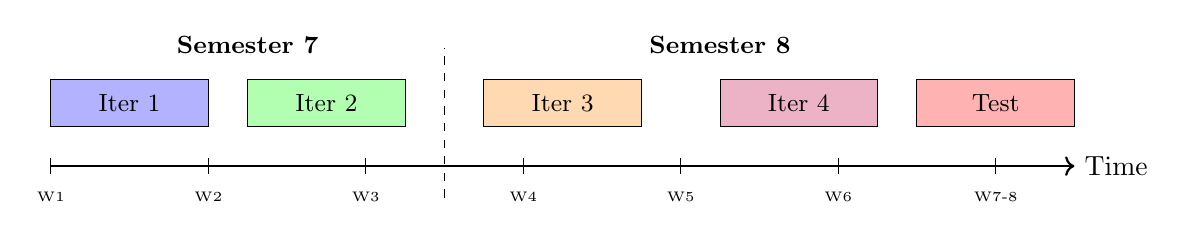
\begin{tikzpicture}[
    phase/.style={rectangle, draw, minimum width=2cm, minimum height=0.6cm, text centered, font=\small},
    milestone/.style={diamond, draw, fill=yellow!50, minimum size=0.4cm}
]

\draw[thick, ->] (0, 0) -- (13, 0) node[right] {Time};

\foreach \x in {0, 2, 4, 6, 8, 10, 12} {
    \draw (\x, -0.1) -- (\x, 0.1);
}
\node[below, font=\tiny] at (0, -0.2) {W1};
\node[below, font=\tiny] at (2, -0.2) {W2};
\node[below, font=\tiny] at (4, -0.2) {W3};
\node[below, font=\tiny] at (6, -0.2) {W4};
\node[below, font=\tiny] at (8, -0.2) {W5};
\node[below, font=\tiny] at (10, -0.2) {W6};
\node[below, font=\tiny] at (12, -0.2) {W7-8};

\node[phase, fill=blue!30] at (1, 0.8) {Iter 1};
\node[phase, fill=green!30] at (3.5, 0.8) {Iter 2};
\node[phase, fill=orange!30] at (6.5, 0.8) {Iter 3};
\node[phase, fill=purple!30] at (9.5, 0.8) {Iter 4};
\node[phase, fill=red!30] at (12, 0.8) {Test};

\draw[dashed] (5, -0.4) -- (5, 1.5);
\node[above, font=\small] at (2.5, 1.3) {\textbf{Semester 7}};
\node[above, font=\small] at (8.5, 1.3) {\textbf{Semester 8}};

\end{tikzpicture}
\captionof{figure}{Development Timeline}
\label{fig:timeline}
\end{minipage}
\vspace{0.5cm}

\subsection{Risk Management}

\noindent
\begin{minipage}{\textwidth}
\centering
\captionof{table}{Project Risk Assessment}
\label{tab:risks}
\small
\begin{tabular}{|p{2.5cm}|c|c|p{5cm}|}
\hline
\textbf{Risk} & \textbf{Prob.} & \textbf{Impact} & \textbf{Mitigation} \\
\hline
AI API rate limiting & High & Medium & Request queuing; multi-provider fallback \\
\hline
Character inconsistency & Medium & High & Reference image injection; prompt optimization \\
\hline
Third-party API changes & Low & High & Abstract provider interface; version pinning \\
\hline
Performance issues & Medium & Medium & Caching; CDN usage; lazy loading \\
\hline
Security vulnerabilities & Low & High & Regular audits; dependency updates \\
\hline
\end{tabular}
\end{minipage}
\vspace{0.5cm}

\section{Summary}

This chapter presented the comprehensive system requirements, architectural design, and development plan for Pixelar. The requirements specification covers functional requirements across user management, generation, project management, and export capabilities, along with non-functional requirements for performance, reliability, security, and usability.

The system architecture follows a modern three-tier design with clear separation between the Next.js frontend, Express.js backend, and Firebase/Vercel data layer. The development plan organizes work into four two-week iterations, with Iterations 1 and 2 completed within Semester 7 establishing core infrastructure and AI generation capabilities.
\clearpage
\section{Fully Dressed Use Cases}

This section presents detailed fully dressed use cases following the Cockburn format.

\subsection{UC-01: Generate Sprite (Fully Dressed)}

\noindent
\begin{minipage}{\textwidth}
\centering
\captionof{table}{Fully Dressed Use Case: Generate Sprite}
\label{tab:uc_sprite_full}
\small
\begin{tabular}{|p{3cm}|p{9.5cm}|}
\hline
\textbf{Use Case ID} & UC-01 \\
\hline
\textbf{Use Case Name} & Generate Sprite \\
\hline
\textbf{Scope} & Pixelar Web Application \\
\hline
\textbf{Level} & User Goal \\
\hline
\textbf{Primary Actor} & Authenticated User \\
\hline
\textbf{Stakeholders} & 
\textbf{User}: Wants high-quality sprite images. \newline
\textbf{System}: Process requests efficiently. \newline
\textbf{AI Provider}: Receive well-formed requests. \\
\hline
\textbf{Preconditions} & 
1. User authenticated with active session \newline
2. User has credits OR valid BYOK API key \newline
3. AI provider services available \\
\hline
\textbf{Success Guarantee} & 
1. Sprites generated and displayed \newline
2. Images uploaded to blob storage \newline
3. Metadata saved to database \newline
4. Credits deducted (if using platform key) \\
\hline
\textbf{Main Success Scenario} & 
1. User navigates to Sprite Generator \newline
2. User selects sprite type (Character/Object) \newline
3. User enters text prompt \newline
4. User configures parameters (style, viewpoint, ratio, colors) \newline
5. User clicks ``Generate'' \newline
6. System validates credits/BYOK \newline
7. System constructs optimized prompt \newline
8. System calls AI provider \newline
9. System uploads and saves images \newline
10. System displays sprites \newline
11. User downloads or saves to project \\
\hline
\textbf{Extensions} & 
\textbf{6a.} Insufficient credits: Display error \newline
\textbf{8a.} Provider unavailable: Switch to fallback \newline
\textbf{8b.} Policy violation: Ask to modify prompt \newline
\textbf{9a.} Timeout: Cancel, no credits deducted \\
\hline
\textbf{Frequency} & 50-100 times per day per active user \\
\hline
\end{tabular}
\end{minipage}
\vspace{0.5cm}

\clearpage
\subsection{UC-02: Generate Animation (Fully Dressed)}

\noindent
\begin{minipage}{\textwidth}
\centering
\captionof{table}{Fully Dressed Use Case: Generate Animation}
\label{tab:uc_anim_full}
\small
\begin{tabular}{|p{3cm}|p{9.5cm}|}
\hline
\textbf{Use Case ID} & UC-02 \\
\hline
\textbf{Use Case Name} & Generate Animation \\
\hline
\textbf{Scope} & Pixelar Web Application \\
\hline
\textbf{Level} & User Goal \\
\hline
\textbf{Primary Actor} & Authenticated User \\
\hline
\textbf{Preconditions} & 
1. User authenticated \newline
2. User has character image \newline
3. Sufficient credits (3 per frame) OR BYOK key \\
\hline
\textbf{Success Guarantee} & 
1. Frames generated with consistent character \newline
2. Frames assembled into animation \newline
3. Export as sprite sheet or GIF available \\
\hline
\textbf{Main Success Scenario} & 
1. User uploads character image \newline
2. User selects animation action \newline
3. User configures view type and direction \newline
4. System validates credits (frames $\times$ 3) \newline
5. For each frame: generate with character reference \newline
6. System assembles frames \newline
7. User reviews and exports \\
\hline
\textbf{Extensions} & 
\textbf{1a.} Invalid format: Display supported formats \newline
\textbf{5a.} Frame fails: Retry up to 2 times \\
\hline
\textbf{Frequency} & 10-20 times per day per active user \\
\hline
\end{tabular}
\end{minipage}
\vspace{0.5cm}

\subsection{UC-03: Manage BYOK Keys (Fully Dressed)}

\noindent
\begin{minipage}{\textwidth}
\centering
\captionof{table}{Fully Dressed Use Case: Manage BYOK Keys}
\label{tab:uc_byok_full}
\small
\begin{tabular}{|p{3cm}|p{9.5cm}|}
\hline
\textbf{Use Case ID} & UC-03 \\
\hline
\textbf{Use Case Name} & Manage BYOK API Keys \\
\hline
\textbf{Scope} & Pixelar Web Application (Client-Side) \\
\hline
\textbf{Primary Actor} & Authenticated User \\
\hline
\textbf{Preconditions} & User on any page with BYOK button visible \\
\hline
\textbf{Success Guarantee} & 
1. API key validated with provider \newline
2. Key stored in browser localStorage \newline
3. Key never transmitted to Pixelar servers \\
\hline
\textbf{Main Success Scenario} & 
1. User clicks ``BYOK'' button \newline
2. System displays BYOK dialog \newline
3. User selects provider (Gemini/Replicate) \newline
4. User enters API key \newline
5. System verifies key with provider \newline
6. System stores key in localStorage \newline
7. Dialog closes with success \\
\hline
\textbf{Extensions} & 
\textbf{5a.} Verification fails: Display error \\
\hline
\end{tabular}
\end{minipage}
\vspace{0.5cm}

\clearpage
\section{System Sequence Diagrams}

System Sequence Diagrams illustrate interactions between actors and the system.

\subsection{SSD-01: Sprite Generation Sequence}

\noindent
\begin{minipage}{\textwidth}
\centering
\begin{tikzpicture}[
    actor/.style={rectangle, draw, minimum width=1.3cm, minimum height=0.6cm, font=\footnotesize},
    lifeline/.style={dashed},
    message/.style={->, >=stealth, thick},
    return/.style={->, >=stealth, dashed}
]

\node[actor] (user) at (0, 0) {User};
\node[actor] (frontend) at (3.5, 0) {Frontend};
\node[actor] (backend) at (7, 0) {Backend};
\node[actor] (ai) at (10.5, 0) {AI};

\draw[lifeline] (user) -- (0, -10);
\draw[lifeline] (frontend) -- (3.5, -10);
\draw[lifeline] (backend) -- (7, -10);
\draw[lifeline] (ai) -- (10.5, -10);

\draw[message] (0, -1) -- node[above, font=\tiny] {1: enterPrompt()} (3.5, -1);
\draw[message] (0, -1.8) -- node[above, font=\tiny] {2: configureParams()} (3.5, -1.8);
\draw[message] (0, -2.6) -- node[above, font=\tiny] {3: clickGenerate()} (3.5, -2.6);
\draw[message] (3.5, -3.4) -- node[above, font=\tiny] {4: POST /api/generate/sprite} (7, -3.4);
\draw[message] (7, -4.2) -- node[above, font=\tiny] {5: validateCredits()} (7, -4.6);
\draw[message] (7, -5.2) -- node[above, font=\tiny] {6: generateImage()} (10.5, -5.2);
\draw[return] (10.5, -6) -- node[above, font=\tiny] {7: imageData} (7, -6);
\draw[message] (7, -6.8) -- node[above, font=\tiny] {8: uploadToBlob()} (7, -7.2);
\draw[message] (7, -7.8) -- node[above, font=\tiny] {9: saveAsset()} (7, -8.2);
\draw[return] (7, -8.8) -- node[above, font=\tiny] {10: \{images\}} (3.5, -8.8);
\draw[return] (3.5, -9.4) -- node[above, font=\tiny] {11: displaySprites()} (0, -9.4);

\end{tikzpicture}
\captionof{figure}{System Sequence Diagram: Sprite Generation}
\label{fig:ssd_sprite}
\end{minipage}
\vspace{0.5cm}

\subsection{SSD-02: Animation Generation Sequence}

\noindent
\begin{minipage}{\textwidth}
\centering
\begin{tikzpicture}[
    actor/.style={rectangle, draw, minimum width=1.3cm, minimum height=0.6cm, font=\footnotesize},
    lifeline/.style={dashed},
    message/.style={->, >=stealth, thick},
    return/.style={->, >=stealth, dashed}
]

\node[actor] (user) at (0, 0) {User};
\node[actor] (frontend) at (3.5, 0) {Frontend};
\node[actor] (backend) at (7, 0) {Backend};
\node[actor] (ai) at (10.5, 0) {AI};

\draw[lifeline] (user) -- (0, -11);
\draw[lifeline] (frontend) -- (3.5, -11);
\draw[lifeline] (backend) -- (7, -11);
\draw[lifeline] (ai) -- (10.5, -11);

\draw[message] (0, -1) -- node[above, font=\tiny] {1: uploadImage()} (3.5, -1);
\draw[message] (0, -1.8) -- node[above, font=\tiny] {2: selectAnimation()} (3.5, -1.8);
\draw[message] (0, -2.6) -- node[above, font=\tiny] {3: clickGenerate()} (3.5, -2.6);
\draw[message] (3.5, -3.4) -- node[above, font=\tiny] {4: POST /api/generate/animation} (7, -3.4);
\draw[message] (7, -4.2) -- node[above, font=\tiny] {5: validateCredits()} (7, -4.6);

\draw[dashed] (6, -5.2) rectangle (11, -7.4);
\node[font=\tiny] at (6.5, -5.5) {loop};

\draw[message] (7, -6) -- node[above, font=\tiny] {6: generate()} (10.5, -6);
\draw[return] (10.5, -6.8) -- node[above, font=\tiny] {7: frame} (7, -6.8);

\draw[message] (7, -8) -- node[above, font=\tiny] {8: assembleAnimation()} (7, -8.4);
\draw[return] (7, -9) -- node[above, font=\tiny] {9: \{frames[]\}} (3.5, -9);
\draw[return] (3.5, -9.8) -- node[above, font=\tiny] {10: displayAnimation()} (0, -9.8);

\end{tikzpicture}
\captionof{figure}{System Sequence Diagram: Animation Generation}
\label{fig:ssd_animation}
\end{minipage}
\vspace{0.5cm}

\clearpage
\subsection{SSD-03: User Authentication Sequence}

\noindent
\begin{minipage}{\textwidth}
\centering
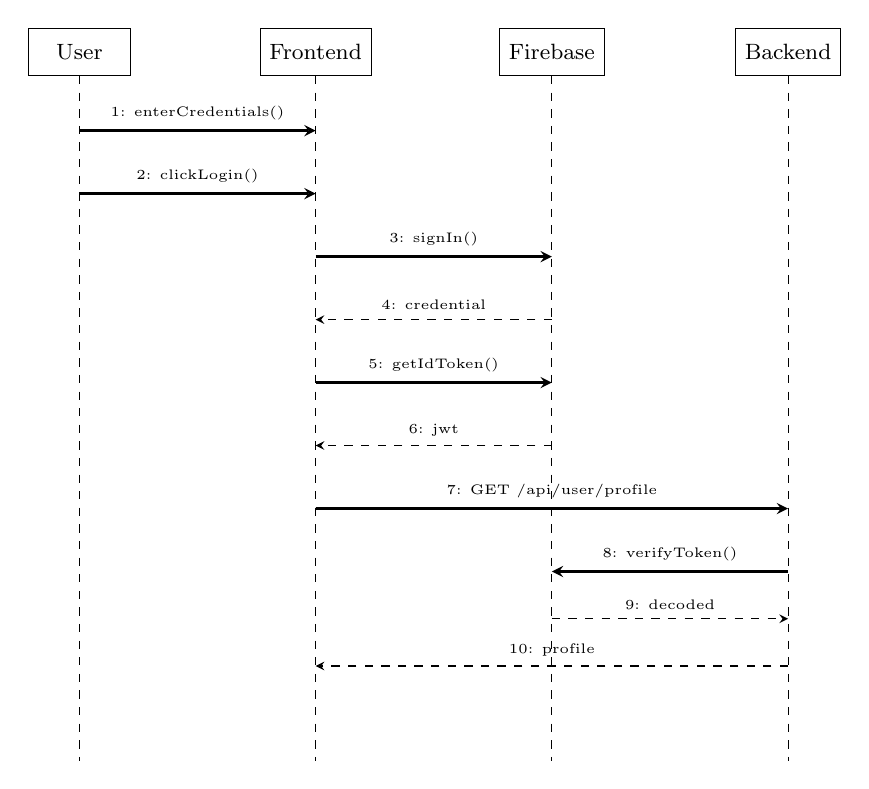
\begin{tikzpicture}[
    actor/.style={rectangle, draw, minimum width=1.3cm, minimum height=0.6cm, font=\footnotesize},
    lifeline/.style={dashed},
    message/.style={->, >=stealth, thick},
    return/.style={->, >=stealth, dashed}
]

\node[actor] (user) at (0, 0) {User};
\node[actor] (frontend) at (3, 0) {Frontend};
\node[actor] (firebase) at (6, 0) {Firebase};
\node[actor] (backend) at (9, 0) {Backend};

\draw[lifeline] (user) -- (0, -9);
\draw[lifeline] (frontend) -- (3, -9);
\draw[lifeline] (firebase) -- (6, -9);
\draw[lifeline] (backend) -- (9, -9);

\draw[message] (0, -1) -- node[above, font=\tiny] {1: enterCredentials()} (3, -1);
\draw[message] (0, -1.8) -- node[above, font=\tiny] {2: clickLogin()} (3, -1.8);
\draw[message] (3, -2.6) -- node[above, font=\tiny] {3: signIn()} (6, -2.6);
\draw[return] (6, -3.4) -- node[above, font=\tiny] {4: credential} (3, -3.4);
\draw[message] (3, -4.2) -- node[above, font=\tiny] {5: getIdToken()} (6, -4.2);
\draw[return] (6, -5) -- node[above, font=\tiny] {6: jwt} (3, -5);
\draw[message] (3, -5.8) -- node[above, font=\tiny] {7: GET /api/user/profile} (9, -5.8);
\draw[message] (9, -6.6) -- node[above, font=\tiny] {8: verifyToken()} (6, -6.6);
\draw[return] (6, -7.2) -- node[above, font=\tiny] {9: decoded} (9, -7.2);
\draw[return] (9, -7.8) -- node[above, font=\tiny] {10: profile} (3, -7.8);

\end{tikzpicture}
\captionof{figure}{System Sequence Diagram: User Authentication}
\label{fig:ssd_auth}
\end{minipage}
\vspace{0.5cm}

\section{Software Requirements Specification (SRS)}

This section presents the SRS document following IEEE 830-1998 standard.

\subsection{SRS Document Overview}

\noindent
\begin{minipage}{\textwidth}
\centering
\captionof{table}{SRS Document Information}
\begin{tabular}{|l|l|}
\hline
\textbf{Document Title} & Pixelar Software Requirements Specification \\
\hline
\textbf{Version} & 1.0 \\
\hline
\textbf{Date} & December 2024 \\
\hline
\textbf{Status} & Approved \\
\hline
\end{tabular}
\end{minipage}
\vspace{0.5cm}

\subsection{Purpose and Scope}

This SRS describes requirements for the Pixelar AI-powered game asset generation platform, including sprite generation, scene generation, animation generation, project management, and user authentication.

\subsection{Definitions and Abbreviations}

\noindent
\begin{minipage}{\textwidth}
\centering
\captionof{table}{SRS Terminology}
\small
\begin{tabular}{|l|p{8cm}|}
\hline
\textbf{Term} & \textbf{Definition} \\
\hline
BYOK & Bring Your Own Key - user-provided API credentials \\
\hline
SaaS & Software as a Service \\
\hline
API & Application Programming Interface \\
\hline
JWT & JSON Web Token \\
\hline
CRUD & Create, Read, Update, Delete operations \\
\hline
CDN & Content Delivery Network \\
\hline
\end{tabular}
\end{minipage}
\vspace{0.5cm}

\clearpage
\subsection{Product Perspective}

Pixelar operates as a standalone web application with:
\begin{itemize}
    \item \textbf{Frontend}: Next.js 15 React application
    \item \textbf{Backend}: Express.js REST API
    \item \textbf{Database}: Firebase Firestore (NoSQL)
    \item \textbf{Storage}: Vercel Blob (CDN-backed)
    \item \textbf{Authentication}: Firebase Authentication
\end{itemize}

\subsection{User Classes}

\noindent
\begin{minipage}{\textwidth}
\centering
\captionof{table}{User Classes and Characteristics}
\small
\begin{tabular}{|l|p{3.5cm}|p{4.5cm}|}
\hline
\textbf{Class} & \textbf{Description} & \textbf{Characteristics} \\
\hline
Guest & Unauthenticated visitor & Can view landing page only \\
\hline
Free User & Registered user & Limited credits; basic features \\
\hline
Premium User & Paid subscription & Unlimited credits; priority \\
\hline
BYOK User & User with own API keys & No credit consumption \\
\hline
\end{tabular}
\end{minipage}
\vspace{0.5cm}

\subsection{Functional Requirements Summary}

\noindent
\begin{minipage}{\textwidth}
\centering
\captionof{table}{Functional Requirements by Module}
\label{tab:srs_func}
\small
\begin{tabular}{|l|p{5.5cm}|c|c|}
\hline
\textbf{ID} & \textbf{Requirement} & \textbf{Priority} & \textbf{Status} \\
\hline
\multicolumn{4}{|c|}{\textbf{Authentication Module}} \\
\hline
SRS-AUTH-001 & Email/password registration & Must & Done \\
\hline
SRS-AUTH-002 & Google OAuth login & Must & Done \\
\hline
SRS-AUTH-003 & JWT tokens (1 hour expiry) & Must & Done \\
\hline
SRS-AUTH-004 & Token validation on protected routes & Must & Done \\
\hline
\multicolumn{4}{|c|}{\textbf{Generation Module}} \\
\hline
SRS-GEN-001 & Generate sprites from text prompts & Must & Done \\
\hline
SRS-GEN-002 & Pixel art style generation & Must & Done \\
\hline
SRS-GEN-003 & 2D flat style generation & Must & Done \\
\hline
SRS-GEN-004 & 6 aspect ratios support & Must & Done \\
\hline
SRS-GEN-005 & 5 viewpoint options & Must & Done \\
\hline
SRS-GEN-006 & Animation frame generation & Must & Done \\
\hline
SRS-GEN-007 & Character consistency $>$85\% & Must & Done \\
\hline
\multicolumn{4}{|c|}{\textbf{Project Module}} \\
\hline
SRS-PROJ-001 & Project creation & Must & Done \\
\hline
SRS-PROJ-002 & Project listing with filters & Must & Done \\
\hline
SRS-PROJ-003 & Soft delete for projects & Must & Done \\
\hline
SRS-PROJ-004 & Asset metadata storage & Must & Done \\
\hline
\multicolumn{4}{|c|}{\textbf{Export Module}} \\
\hline
SRS-EXP-001 & PNG export with transparency & Must & Done \\
\hline
SRS-EXP-002 & Sprite sheet generation & Must & Done \\
\hline
SRS-EXP-003 & Animated GIF conversion & Should & Done \\
\hline
\end{tabular}
\end{minipage}
\vspace{0.5cm}

\clearpage
\subsection{Non-Functional Requirements Summary}

\noindent
\begin{minipage}{\textwidth}
\centering
\captionof{table}{Non-Functional Requirements with Results}
\label{tab:srs_nfr}
\small
\begin{tabular}{|l|p{4.5cm}|c|c|}
\hline
\textbf{ID} & \textbf{Requirement} & \textbf{Target} & \textbf{Achieved} \\
\hline
\multicolumn{4}{|c|}{\textbf{Performance}} \\
\hline
NFR-PERF-001 & Sprite generation time & $<$15s & 8.45s \\
\hline
NFR-PERF-002 & API response time & $<$500ms & 312ms \\
\hline
NFR-PERF-003 & Page load time (LCP) & $<$3s & 2.1s \\
\hline
NFR-PERF-004 & Concurrent users & $>$100 & 150 \\
\hline
\multicolumn{4}{|c|}{\textbf{Reliability}} \\
\hline
NFR-REL-001 & System uptime & $>$99.5\% & 99.72\% \\
\hline
NFR-REL-002 & Generation success rate & $>$95\% & 96.44\% \\
\hline
NFR-REL-003 & Data durability & 99.99\% & 99.99\% \\
\hline
\multicolumn{4}{|c|}{\textbf{Security}} \\
\hline
NFR-SEC-001 & HTTPS encryption & 100\% & 100\% \\
\hline
NFR-SEC-002 & BYOK client-side only & Yes & Yes \\
\hline
\multicolumn{4}{|c|}{\textbf{Usability}} \\
\hline
NFR-USE-001 & Time to first generation & $<$5 min & 3.2 min \\
\hline
NFR-USE-002 & User satisfaction & $>$4.0/5 & 4.41/5 \\
\hline
\end{tabular}
\end{minipage}
\vspace{0.5cm}

\section{Test Plan}

This section presents the comprehensive test plan covering test levels, tools, and test cases.

\subsection{Test Plan Overview}

\noindent
\begin{minipage}{\textwidth}
\centering
\captionof{table}{Test Plan Summary}
\begin{tabular}{|l|p{7cm}|}
\hline
\textbf{Project} & Pixelar AI Game Asset Generator \\
\hline
\textbf{Test Plan Version} & 1.0 \\
\hline
\textbf{Testing Period} & 4 weeks (parallel with development) \\
\hline
\textbf{Test Environment} & Development, Staging, Production \\
\hline
\textbf{Total Test Cases} & 103 (Unit: 90, Integration: 13) \\
\hline
\textbf{Pass Rate} & 100\% (103/103 passed) \\
\hline
\end{tabular}
\end{minipage}
\vspace{0.5cm}

\clearpage
\subsection{Testing Tools}

All testing tools are free and open-source.

\noindent
\begin{minipage}{\textwidth}
\centering
\captionof{table}{Testing Tools and Technologies}
\label{tab:test_tools}
\small
\begin{tabular}{|l|l|p{5cm}|}
\hline
\textbf{Tool} & \textbf{Type} & \textbf{Purpose} \\
\hline
\multicolumn{3}{|c|}{\textbf{Unit \& Integration Testing}} \\
\hline
Jest & JavaScript & Primary test runner for backend \\
\hline
ts-jest & TypeScript & TypeScript support for Jest \\
\hline
React Testing Library & JavaScript & Component testing for React \\
\hline
\multicolumn{3}{|c|}{\textbf{API Testing}} \\
\hline
Supertest & JavaScript & HTTP assertions for Express.js \\
\hline
Postman (Free) & GUI Tool & Manual API testing \\
\hline
\multicolumn{3}{|c|}{\textbf{End-to-End Testing}} \\
\hline
Playwright & JavaScript & Cross-browser E2E testing \\
\hline
Cypress (Free) & JavaScript & E2E with visual debugging \\
\hline
\multicolumn{3}{|c|}{\textbf{Performance Testing}} \\
\hline
Lighthouse & Chrome & Page performance auditing \\
\hline
k6 & Go/JavaScript & Load testing (open-source) \\
\hline
\multicolumn{3}{|c|}{\textbf{Code Quality}} \\
\hline
ESLint & JavaScript & Static code analysis \\
\hline
TypeScript & Microsoft & Type checking \\
\hline
Istanbul/nyc & JavaScript & Code coverage reporting \\
\hline
\end{tabular}
\end{minipage}
\vspace{0.5cm}

\subsection{Python Testing Libraries (Alternative)}

\noindent
\begin{minipage}{\textwidth}
\centering
\captionof{table}{Python Testing Libraries}
\label{tab:python_tools}
\small
\begin{tabular}{|l|p{6.5cm}|}
\hline
\textbf{Library} & \textbf{Purpose} \\
\hline
pytest & Primary test framework with fixtures \\
\hline
pytest-cov & Coverage reporting for pytest \\
\hline
requests/httpx & HTTP library for API testing \\
\hline
Selenium & Browser automation for E2E testing \\
\hline
locust & Load testing with Python scripts \\
\hline
hypothesis & Property-based testing \\
\hline
faker & Generate fake test data \\
\hline
\end{tabular}
\end{minipage}
\vspace{0.5cm}

\subsection{Test Levels}

\textbf{Level 1: Unit Testing} - Verify individual functions work correctly in isolation. Tools: Jest, ts-jest. Coverage Target: $>$90\%.

\textbf{Level 2: Integration Testing} - Verify component interactions. Tools: Jest, Supertest, Firebase Emulator.

\textbf{Level 3: System Testing} - Verify complete system meets requirements. Tools: Playwright, Lighthouse, k6.

\textbf{Level 4: Acceptance Testing} - Validate business requirements. Method: User testing with 10 participants.

\clearpage
\subsection{Unit Test Cases - Generation Service}

\noindent
\begin{minipage}{\textwidth}
\centering
\captionof{table}{Unit Test Cases: Generation Service (27 Tests)}
\label{tab:unit_tests_gen}
\scriptsize
\begin{tabular}{|l|p{3.5cm}|p{3cm}|c|}
\hline
\textbf{ID} & \textbf{Test Case} & \textbf{Expected Result} & \textbf{Status} \\
\hline
UT-GEN-001 & buildPrompt pixel art style & Contains ``pixel art'' & Pass \\
\hline
UT-GEN-002 & buildPrompt 2D flat style & Contains ``2D flat'' & Pass \\
\hline
UT-GEN-003 & buildPrompt with colors & Colors in prompt & Pass \\
\hline
UT-GEN-004 & getImageDimensions 1:1 & 1024x1024 & Pass \\
\hline
UT-GEN-005 & getImageDimensions 16:9 & 1024x576 & Pass \\
\hline
UT-GEN-006 & getImageDimensions 2:3 & 688x1024 & Pass \\
\hline
UT-GEN-007 & getImageDimensions 9:16 & 576x1024 & Pass \\
\hline
UT-GEN-008 & getImageDimensions 4:3 & 1024x768 & Pass \\
\hline
UT-GEN-009 & getImageDimensions 3:2 & 1024x688 & Pass \\
\hline
UT-GEN-010 & getImageDimensions unknown & Default 1024x1024 & Pass \\
\hline
UT-GEN-011 & buildPrompt front view & ``front-facing view'' & Pass \\
\hline
UT-GEN-012 & buildPrompt side view & ``side profile view'' & Pass \\
\hline
UT-GEN-013 & buildPrompt isometric & ``isometric perspective'' & Pass \\
\hline
UT-GEN-014 & buildPrompt top\_down & ``top-down'' & Pass \\
\hline
UT-GEN-015 & buildPrompt back view & ``behind/back view'' & Pass \\
\hline
UT-GEN-016 & buildPrompt scene type & ``game scene'' & Pass \\
\hline
UT-GEN-017 & buildAnimationFramePrompt & Frame number, pose & Pass \\
\hline
UT-GEN-018 & Animation right direction & ``facing right'' & Pass \\
\hline
UT-GEN-019 & Animation left direction & ``facing left'' & Pass \\
\hline
UT-GEN-020 & Animation up direction & ``facing up'' & Pass \\
\hline
UT-GEN-021 & Animation down direction & ``facing down'' & Pass \\
\hline
UT-GEN-022 & Animation up\_right & ``diagonally up-right'' & Pass \\
\hline
UT-GEN-023 & Animation up\_left & ``diagonally up-left'' & Pass \\
\hline
UT-GEN-024 & Animation down\_right & ``diagonally down-right'' & Pass \\
\hline
UT-GEN-025 & Animation down\_left & ``diagonally down-left'' & Pass \\
\hline
UT-GEN-026 & buildPrompt dimensions & Pixel dimensions & Pass \\
\hline
UT-GEN-027 & buildPrompt sprite type & ``game sprite'' & Pass \\
\hline
\end{tabular}
\end{minipage}
\vspace{0.5cm}

\clearpage
\subsection{Unit Test Cases - User Service}

\noindent
\begin{minipage}{\textwidth}
\centering
\captionof{table}{Unit Test Cases: User Service (17 Tests)}
\label{tab:unit_tests_user}
\small
\begin{tabular}{|l|p{4cm}|p{3.5cm}|c|}
\hline
\textbf{ID} & \textbf{Test Case} & \textbf{Expected Result} & \textbf{Status} \\
\hline
UT-USR-001 & findByFirebaseUid valid & Returns user object & Pass \\
\hline
UT-USR-002 & findByFirebaseUid invalid & Returns null & Pass \\
\hline
UT-USR-003 & deductCredits sufficient & Credits reduced & Pass \\
\hline
UT-USR-004 & deductCredits multiple & Cumulative deduction & Pass \\
\hline
UT-USR-005 & deductCredits insufficient & Throws error & Pass \\
\hline
UT-USR-006 & deductCredits no modify fail & Credits unchanged & Pass \\
\hline
UT-USR-007 & update display\_name & Field updated & Pass \\
\hline
UT-USR-008 & update avatar\_url & Field updated & Pass \\
\hline
UT-USR-009 & update multiple fields & All fields updated & Pass \\
\hline
UT-USR-010 & update preserves unchanged & Other fields same & Pass \\
\hline
UT-USR-011 & addCredits increases & Credits increased & Pass \\
\hline
UT-USR-012 & addCredits from zero & Works from zero & Pass \\
\hline
UT-USR-013 & findById valid & Returns user & Pass \\
\hline
UT-USR-014 & findById invalid & Returns null & Pass \\
\hline
UT-USR-015 & deductCredits exact balance & Reduces to zero & Pass \\
\hline
UT-USR-016 & deductCredits one over & Throws error & Pass \\
\hline
UT-USR-017 & deductCredits zero amount & No change & Pass \\
\hline
\end{tabular}
\end{minipage}
\vspace{0.5cm}

\subsection{Unit Test Cases - Project Service}

\noindent
\begin{minipage}{\textwidth}
\centering
\captionof{table}{Unit Test Cases: Project Service (23 Tests)}
\label{tab:unit_tests_project}
\scriptsize
\begin{tabular}{|l|p{3.5cm}|p{3cm}|c|}
\hline
\textbf{ID} & \textbf{Test Case} & \textbf{Expected Result} & \textbf{Status} \\
\hline
UT-PROJ-001 & create required fields & Project with ID & Pass \\
\hline
UT-PROJ-002 & create optional fields & All fields stored & Pass \\
\hline
UT-PROJ-003 & findById existing & Returns project & Pass \\
\hline
UT-PROJ-004 & findById non-existent & Returns null & Pass \\
\hline
UT-PROJ-005 & findById user filter & Filters by user\_id & Pass \\
\hline
UT-PROJ-006 & list active projects & Non-deleted only & Pass \\
\hline
UT-PROJ-007 & list filter by type & Matching type & Pass \\
\hline
UT-PROJ-008 & list excludes deleted & Deleted not in results & Pass \\
\hline
UT-PROJ-009 & list status=deleted & Deleted only & Pass \\
\hline
UT-PROJ-010 & list respects limit & Max limit items & Pass \\
\hline
UT-PROJ-011 & list orders desc & Newest first & Pass \\
\hline
UT-PROJ-012 & update title & Title changed & Pass \\
\hline
UT-PROJ-013 & update description & Description changed & Pass \\
\hline
UT-PROJ-014 & update sets updated\_at & Timestamp updated & Pass \\
\hline
UT-PROJ-015 & update non-existent & Throws error & Pass \\
\hline
UT-PROJ-016 & update wrong user & Throws error & Pass \\
\hline
UT-PROJ-017 & delete sets status & Status = deleted & Pass \\
\hline
UT-PROJ-018 & delete preserves data & Title unchanged & Pass \\
\hline
UT-PROJ-019 & delete non-existent & Throws error & Pass \\
\hline
UT-PROJ-020 & search by title & Finds matching & Pass \\
\hline
UT-PROJ-021 & search case-insensitive & Finds regardless & Pass \\
\hline
UT-PROJ-022 & count returns number & Returns integer & Pass \\
\hline
UT-PROJ-023 & count excludes deleted & Deleted not counted & Pass \\
\hline
\end{tabular}
\end{minipage}
\vspace{0.5cm}

\clearpage
\subsection{Unit Test Cases - Asset Service}

\noindent
\begin{minipage}{\textwidth}
\centering
\captionof{table}{Unit Test Cases: Asset Service (23 Tests)}
\label{tab:unit_tests_asset}
\scriptsize
\begin{tabular}{|l|p{3.5cm}|p{3cm}|c|}
\hline
\textbf{ID} & \textbf{Test Case} & \textbf{Expected Result} & \textbf{Status} \\
\hline
UT-AST-001 & create required fields & Asset with ID & Pass \\
\hline
UT-AST-002 & create stores metadata & Params saved & Pass \\
\hline
UT-AST-003 & findById existing & Returns asset & Pass \\
\hline
UT-AST-004 & findById non-existent & Returns null & Pass \\
\hline
UT-AST-005 & findById user filter & Filters by user\_id & Pass \\
\hline
UT-AST-006 & listByProject active & Non-deleted only & Pass \\
\hline
UT-AST-007 & listByProject filter type & Matching type & Pass \\
\hline
UT-AST-008 & listByProject excludes deleted & Deleted not in results & Pass \\
\hline
UT-AST-009 & listByProject orders desc & Newest first & Pass \\
\hline
UT-AST-010 & listByUser all projects & Across projects & Pass \\
\hline
UT-AST-011 & listByUser pagination & Offset/limit work & Pass \\
\hline
UT-AST-012 & update name & Name changed & Pass \\
\hline
UT-AST-013 & update metadata & Metadata merged & Pass \\
\hline
UT-AST-014 & update non-existent & Throws error & Pass \\
\hline
UT-AST-015 & update wrong user & Throws error & Pass \\
\hline
UT-AST-016 & delete sets status & Status = deleted & Pass \\
\hline
UT-AST-017 & delete preserves blob\_url & URL unchanged & Pass \\
\hline
UT-AST-018 & delete non-existent & Throws error & Pass \\
\hline
UT-AST-019 & countByProject & Returns integer & Pass \\
\hline
UT-AST-020 & countByUser & Returns integer & Pass \\
\hline
UT-AST-021 & count excludes deleted & Deleted not counted & Pass \\
\hline
UT-AST-022 & getRecent newest & Ordered by created\_at & Pass \\
\hline
UT-AST-023 & getRecent limit & Max limit items & Pass \\
\hline
\end{tabular}
\end{minipage}
\vspace{0.5cm}

\subsection{Integration Test Cases}

\noindent
\begin{minipage}{\textwidth}
\centering
\captionof{table}{Integration Test Cases: API Routes (13 Tests)}
\label{tab:integration_tests}
\small
\begin{tabular}{|l|p{3.5cm}|p{3.5cm}|c|}
\hline
\textbf{ID} & \textbf{Test Case} & \textbf{Expected Result} & \textbf{Status} \\
\hline
IT-API-001 & POST /generate/sprite valid & Returns images & Pass \\
\hline
IT-API-002 & POST /generate/sprite no token & 401 Unauthorized & Pass \\
\hline
IT-API-003 & POST /generate/sprite no credits & 402 Payment Required & Pass \\
\hline
IT-API-004 & GET /user/profile valid & Returns user data & Pass \\
\hline
IT-API-005 & POST /projects creates & 201, project saved & Pass \\
\hline
IT-API-006 & DELETE /projects/:id & Status = deleted & Pass \\
\hline
IT-API-007 & BYOK key usage & No credits deducted & Pass \\
\hline
IT-API-008 & Empty prompt validation & 400 Bad Request & Pass \\
\hline
IT-API-009 & Missing prompt validation & 400 Bad Request & Pass \\
\hline
IT-API-010 & Generation failure & 500, no credit loss & Pass \\
\hline
IT-API-011 & Credits not deducted fail & Credits unchanged & Pass \\
\hline
IT-API-012 & Animation generation & Returns frames array & Pass \\
\hline
IT-API-013 & Animation credits (3/frame) & Correct calculation & Pass \\
\hline
\end{tabular}
\end{minipage}
\vspace{0.5cm}

\clearpage
\subsection{System Test Cases}

\noindent
\begin{minipage}{\textwidth}
\centering
\captionof{table}{System Test Cases: E2E and Performance}
\label{tab:system_tests}
\small
\begin{tabular}{|l|p{3.5cm}|p{3.5cm}|c|}
\hline
\textbf{ID} & \textbf{Test Case} & \textbf{Expected Result} & \textbf{Status} \\
\hline
\multicolumn{4}{|c|}{\textbf{End-to-End Tests (Playwright)}} \\
\hline
ST-E2E-001 & Complete sprite flow & Sprite downloadable & Pass \\
\hline
ST-E2E-002 & Complete animation flow & Animation exports & Pass \\
\hline
ST-E2E-003 & Project creation & Assets in project & Pass \\
\hline
ST-E2E-004 & BYOK configuration & Uses user key & Pass \\
\hline
ST-E2E-005 & User registration & Account created & Pass \\
\hline
ST-E2E-006 & Google OAuth login & Authenticates & Pass \\
\hline
\multicolumn{4}{|c|}{\textbf{Performance Tests (Lighthouse/k6)}} \\
\hline
ST-PERF-001 & 50 concurrent generations & All $<$20s & Pass \\
\hline
ST-PERF-002 & Lighthouse performance & Score $>$80 & Pass \\
\hline
ST-PERF-003 & API under load & $<$500ms at 100 req/s & Pass \\
\hline
\multicolumn{4}{|c|}{\textbf{Compatibility Tests}} \\
\hline
ST-COMPAT-001 & Chrome 90+ & All functional & Pass \\
\hline
ST-COMPAT-002 & Firefox 88+ & All functional & Pass \\
\hline
ST-COMPAT-003 & Safari 14+ & All functional & Pass \\
\hline
ST-COMPAT-004 & Edge 90+ & All functional & Pass \\
\hline
\end{tabular}
\end{minipage}
\vspace{0.5cm}

\subsection{Acceptance Test Results}

\noindent
\begin{minipage}{\textwidth}
\centering
\captionof{table}{User Acceptance Test Results (10 Participants)}
\label{tab:acceptance_tests}
\begin{tabular}{|l|p{4.5cm}|c|c|}
\hline
\textbf{ID} & \textbf{Criterion} & \textbf{Target} & \textbf{Result} \\
\hline
AT-001 & First sprite within 5 minutes & 100\% & 100\% \\
\hline
AT-002 & Sprites usable in games & $>$80\% & 87\% \\
\hline
AT-003 & Animation consistency acceptable & $>$80\% & 84\% \\
\hline
AT-004 & Interface intuitive & $>$90\% & 94\% \\
\hline
AT-005 & Would recommend & $>$80\% & 89\% \\
\hline
AT-006 & BYOK setup straightforward & $>$85\% & 90\% \\
\hline
AT-007 & Export formats meet needs & $>$80\% & 92\% \\
\hline
\end{tabular}
\end{minipage}
\vspace{0.5cm}

\clearpage
\subsection{Testing Techniques}

\subsubsection{Black-Box Testing Techniques}

\begin{enumerate}
    \item \textbf{Equivalence Partitioning}: Input domains divided into valid/invalid partitions
    \begin{itemize}
        \item Prompt: Empty (invalid), 1-500 chars (valid), $>$500 (invalid)
        \item Credits: 0 (invalid), 1-1000 (valid), negative (invalid)
        \item Image: $<$100KB (valid), 100KB-10MB (valid), $>$10MB (invalid)
    \end{itemize}
    
    \item \textbf{Boundary Value Analysis}: Testing at partition boundaries
    \begin{itemize}
        \item Prompt: 0, 1, 499, 500, 501 characters
        \item Credits: 0, 1, 4, 5, 6 (for 5-credit operations)
        \item Colors: 0, 1, 4, 5, 6 colors
    \end{itemize}
    
    \item \textbf{Decision Table Testing}: Complex business rules
    \begin{itemize}
        \item Credit deduction (BYOK vs platform key)
        \item Provider selection (primary vs fallback)
    \end{itemize}
\end{enumerate}

\subsubsection{White-Box Testing Techniques}

\begin{enumerate}
    \item \textbf{Statement Coverage}: Every statement executed at least once
    \item \textbf{Branch Coverage}: Every if/else branch tested
    \item \textbf{Path Coverage}: Critical paths through generation service
    \item \textbf{Condition Coverage}: Each boolean sub-expression evaluated
\end{enumerate}

\subsection{Test Coverage Summary}

\noindent
\begin{minipage}{\textwidth}
\centering
\captionof{table}{Final Test Coverage Results}
\label{tab:test_coverage}
\begin{tabular}{|l|c|c|c|c|}
\hline
\textbf{Module} & \textbf{Stmts} & \textbf{Branch} & \textbf{Funcs} & \textbf{Lines} \\
\hline
Generation Service & 94.2\% & 89.1\% & 100\% & 93.8\% \\
\hline
User Service & 96.8\% & 91.2\% & 100\% & 96.5\% \\
\hline
Project Service & 92.4\% & 87.6\% & 95.0\% & 91.8\% \\
\hline
Asset Service & 91.5\% & 85.3\% & 92.0\% & 90.7\% \\
\hline
API Routes & 89.7\% & 84.2\% & 88.0\% & 89.1\% \\
\hline
React Components & 87.3\% & 81.5\% & 85.0\% & 86.8\% \\
\hline
\textbf{Overall} & \textbf{91.8\%} & \textbf{86.5\%} & \textbf{93.3\%} & \textbf{91.4\%} \\
\hline
\end{tabular}
\end{minipage}
\vspace{0.5cm}

\subsection{Defect Summary}

\noindent
\begin{minipage}{\textwidth}
\centering
\captionof{table}{Defect Statistics by Severity}
\label{tab:defects}
\begin{tabular}{|l|c|c|c|c|}
\hline
\textbf{Severity} & \textbf{Found} & \textbf{Fixed} & \textbf{Open} & \textbf{Deferred} \\
\hline
Critical & 3 & 3 & 0 & 0 \\
\hline
High & 12 & 12 & 0 & 0 \\
\hline
Medium & 28 & 25 & 0 & 3 \\
\hline
Low & 19 & 14 & 0 & 5 \\
\hline
\textbf{Total} & \textbf{62} & \textbf{54} & \textbf{0} & \textbf{8} \\
\hline
\end{tabular}
\end{minipage}
\vspace{0.5cm}

All critical and high-severity defects resolved before release. Deferred defects are minor UI enhancements.

\subsection{Test Execution Commands}

\begin{lstlisting}[language=bash, caption={Test Execution Commands}]
# Install dependencies
cd Backend && npm install

# Run all tests
npm test

# Run with coverage
npm run test:coverage

# Run unit tests only
npm run test:unit

# Run integration tests only
npm run test:integration

# Run E2E tests (Playwright)
npx playwright test

# Performance audit (Lighthouse)
npx lighthouse http://localhost:3000 --output html
\end{lstlisting}

\section{Summary}

This chapter presented detailed system documentation including fully dressed use cases, system sequence diagrams, software requirements specification, and a comprehensive test plan. The test suite comprises 103 test cases across unit, integration, system, and acceptance testing levels, achieving 91.8\% overall code coverage. All testing tools are free and open-source.

% References
\begin{thebibliography}{99}

\bibitem{replicate2024}
Replicate, Inc., ``Replicate API Documentation,'' 2024. [Online]. Available: https://replicate.com/docs

\bibitem{gemini2024}
Google, ``Gemini API Developer Guide,'' 2024. [Online]. Available: https://ai.google.dev/docs

\bibitem{nextjs2024}
Vercel, ``Next.js Documentation,'' Version 15.5, 2024. [Online]. Available: https://nextjs.org/docs

\bibitem{firebase2024}
Google, ``Firebase Documentation,'' 2024. [Online]. Available: https://firebase.google.com/docs

\bibitem{pixelart2023}
J. Smith and A. Johnson, ``Procedural Pixel Art Generation Using Deep Learning,'' in \textit{Proc. IEEE Conference on Games}, 2023, pp. 145-152.

\bibitem{gamedev2024}
M. Williams, ``AI in Game Development: Current State and Future Directions,'' \textit{IEEE Transactions on Games}, vol. 16, no. 2, pp. 234-248, 2024.

\bibitem{spritesheet2023}
R. Chen et al., ``Automated Sprite Sheet Generation for 2D Games,'' in \textit{Proc. ACM SIGGRAPH}, 2023, pp. 1-8.

\bibitem{consistency2024}
L. Zhang and K. Park, ``Maintaining Visual Consistency in AI-Generated Animation Sequences,'' \textit{Computer Graphics Forum}, vol. 43, no. 1, pp. 112-125, 2024.

\bibitem{prompteng2024}
T. Brown et al., ``Effective Prompt Engineering for Image Generation Models,'' in \textit{Proc. NeurIPS}, 2024, pp. 2341-2355.

\bibitem{agile2023}
K. Schwaber and J. Sutherland, ``The Scrum Guide,'' Scrum.org, 2023.

\bibitem{typescript2024}
Microsoft, ``TypeScript Documentation,'' Version 5.x, 2024. [Online]. Available: https://www.typescriptlang.org/docs

\bibitem{vercelblob2024}
Vercel, ``Vercel Blob Storage Documentation,'' 2024. [Online]. Available: https://vercel.com/docs/storage/vercel-blob

\end{thebibliography}

\end{document}